% Chapter2

\chapter{State of the Art} \label{chapter:stateoftheart}

	\section{Konzeptionelle Planung einer Anlage}
	Es ist gängige Praxis in der Anlagen- und Verfahrenstechnik, vor Realisierung der Anlage eine schematische Darstellung zu modellieren. Das \acf{RI} ist ein probates Mittel für die Erstellung eines vollständiges Abbildes. Die verwendeten Bauteile sind jedenfalls namentlich beschriftet, können aber auch zusätzliche Informationen, die zum Verständnis der Verwendung beitragen, beinhalten. Das beschriebene Schema unterliegt dem Standard DIN EN ISO 10628. Weitere Rohrleitungssymbole können der DIN 2429 entnommen werden.\\

	Zur Anwendung kommt der beschriebene Arbeitsschritt beispielsweise bei einem Reaktor, welcher die hinreichende Bedingung \glqq Name \grqq \space und darüber hinaus fakultative Invarianten wie Anzahl und Lokalisation der Ein- und Ausgänge hat. Weiteres könnten auch Angaben zur Implementierung von Sensoren oder Aktoren vermerkt sein. Rohre werden im \ac{RI} als Verbindungslinien zwischen Bauteilen dargestellt. Detailinformationen wie Nenndruck, Rohrklasse oder Spezifikationsnummer können ergänzend vermerkt werden. Somit sind in einem \ac{RI} Apparate (Tanks, Speicherbehälter, Reaktoren, o. Ä.), Maschinen (Pumpen, Verdichter, o. Ä.) und Leitungen darstellbar.\\
	
	Die folgende Abbildung~\ref{fig:RI_SotA} zeigt den Aufbau einer simplen Anlage mit Hilfe des \ac{RI}.\\

	\begin{figure}[h!]
  		\centering
		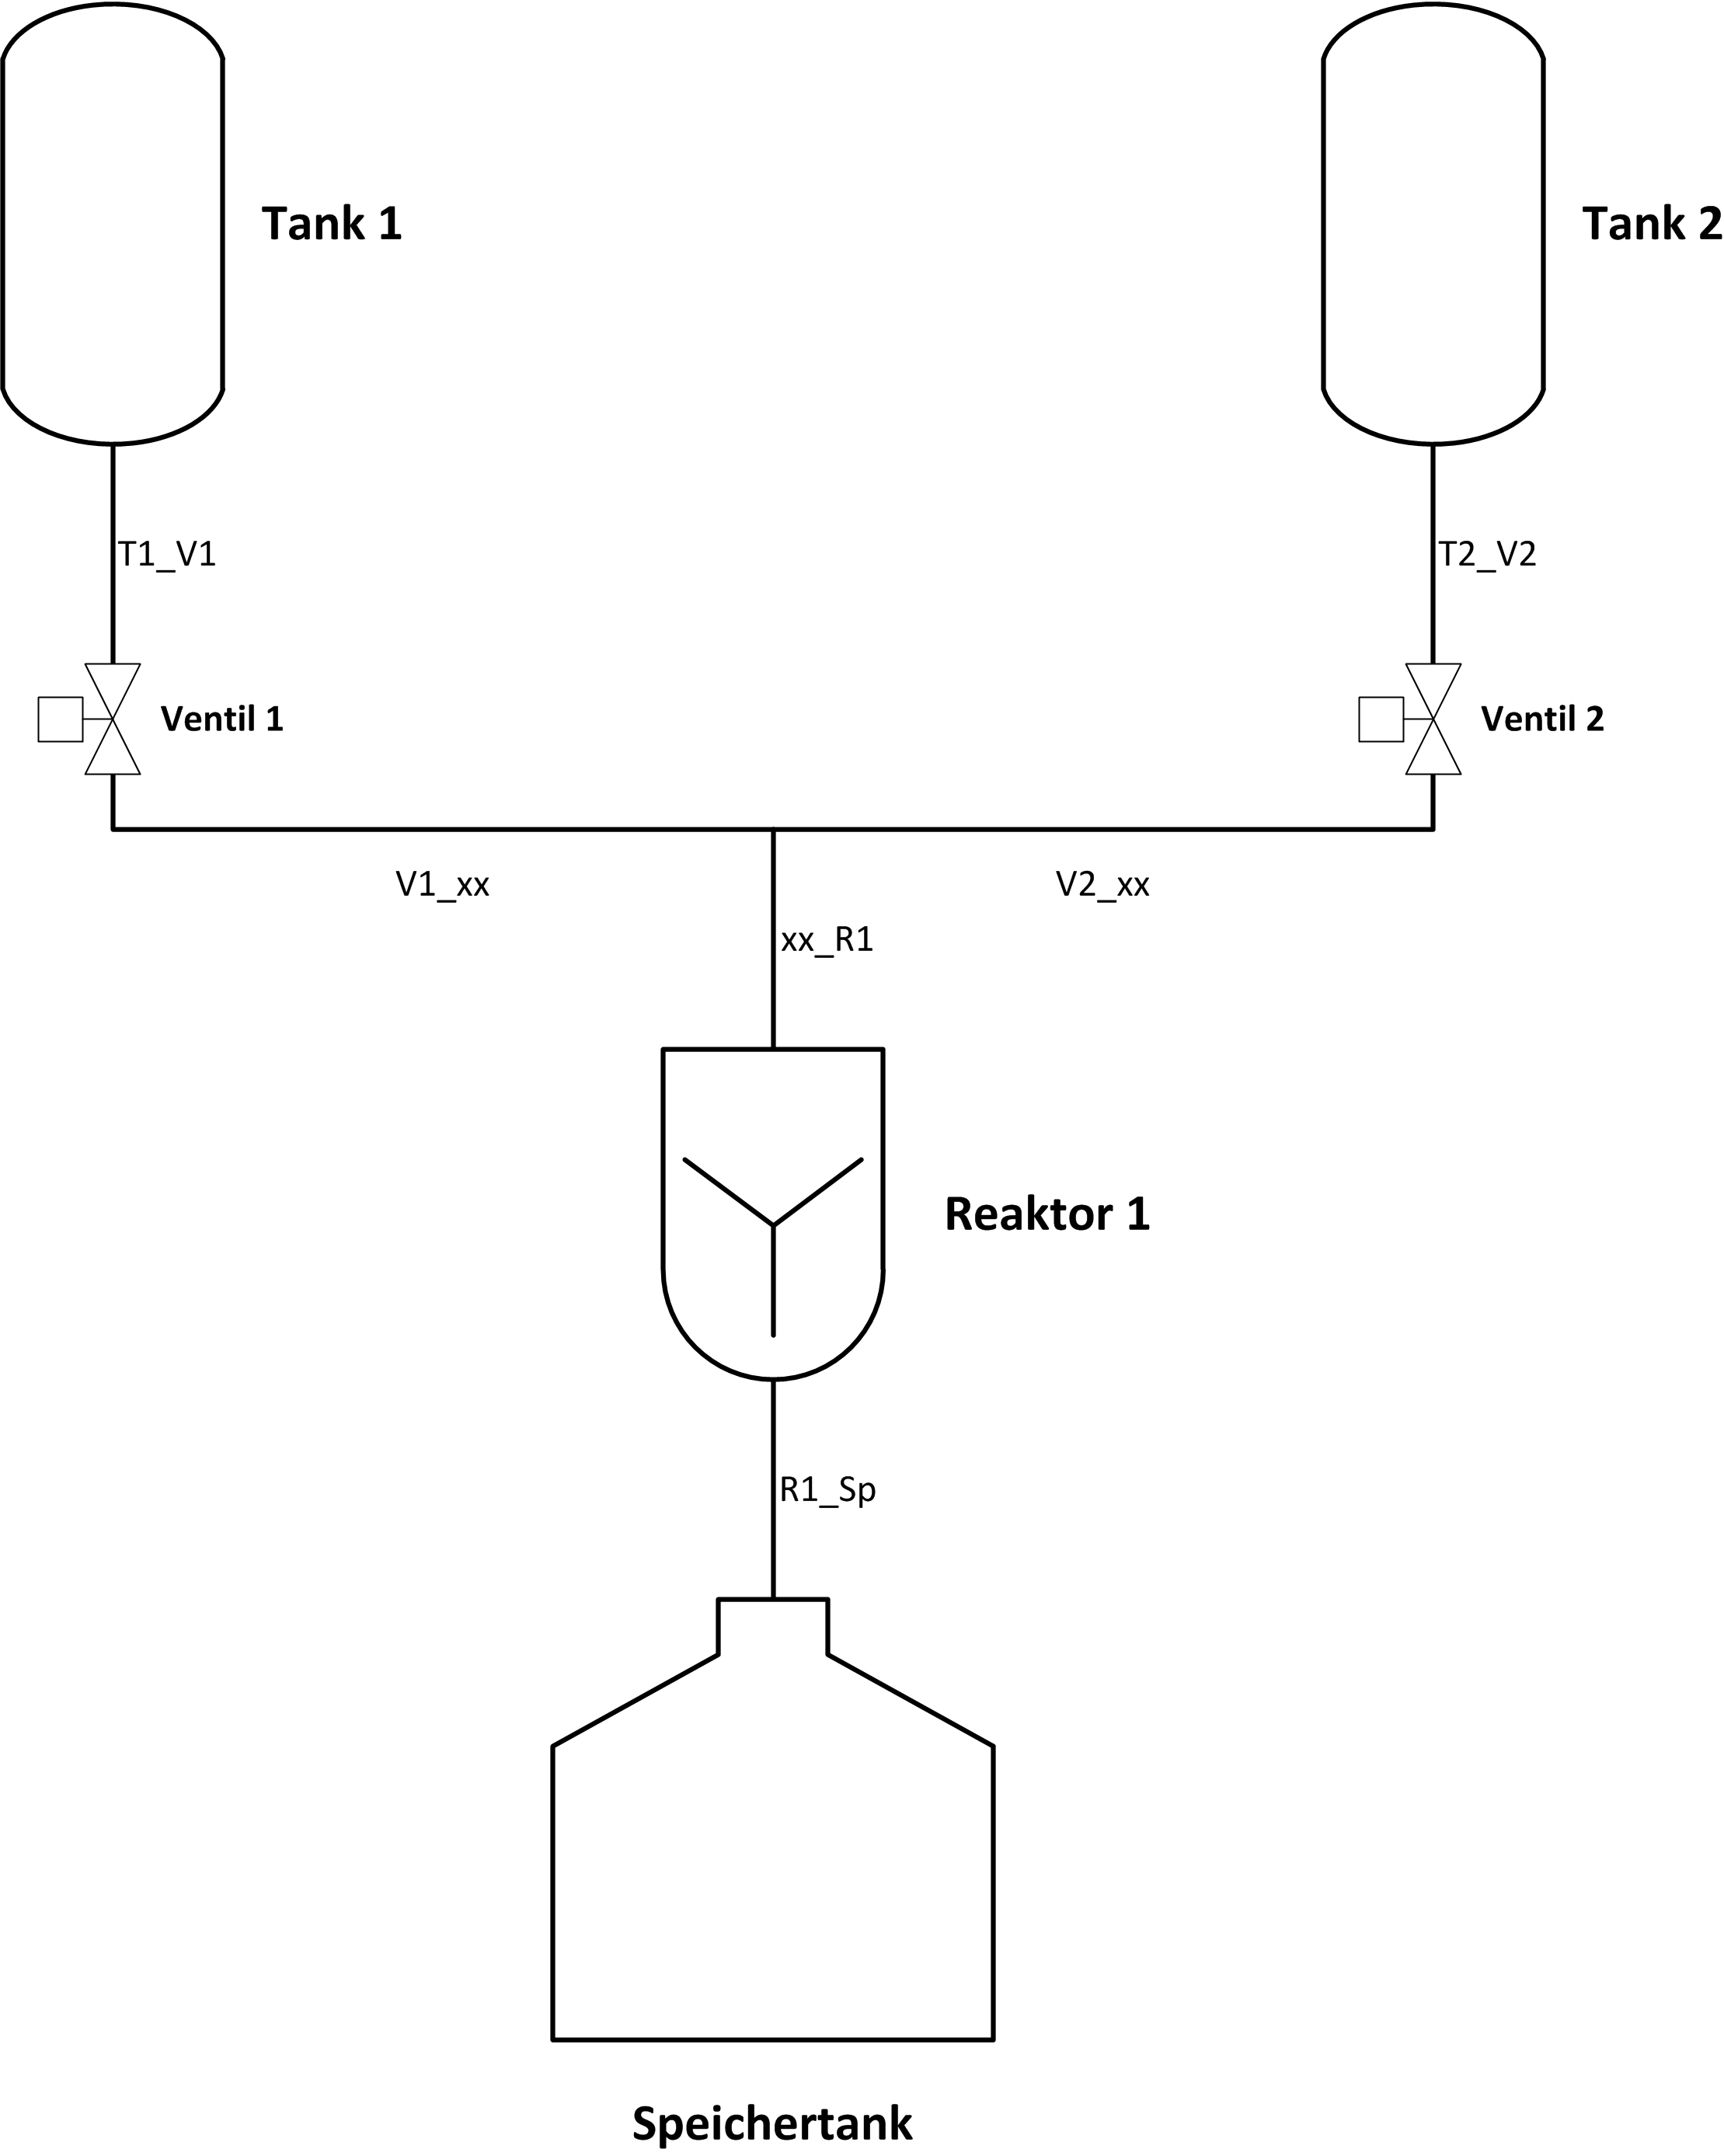
\includegraphics[height=0.7\textwidth]{graphics/stateoftheart/RI_SotA.jpg}
		\caption{Rohr- und Instrumentenfließschema}
		\label{fig:RI_SotA}
	\end{figure}

	\newpage
	\section{Definition eines Prozesses}
	Ein Prozess ist dadurch definiert, welche Arbeitsschritte bewerkstelligt werden müssen, um als Ergebnis das gewünschte Produkt zu erlangen. Die Anforderungen beziehungsweise das Zielprodukt formt somit den Arbeitsprozess. Zu beachten ist, dass diese Verbindung unidirektional ist, da Produkte nicht auf Basis der Prozesse definiert werden (siehe Abbildung~\ref{fig:prozessdef}).
	
	\begin{figure}[h!]
  		\centering
		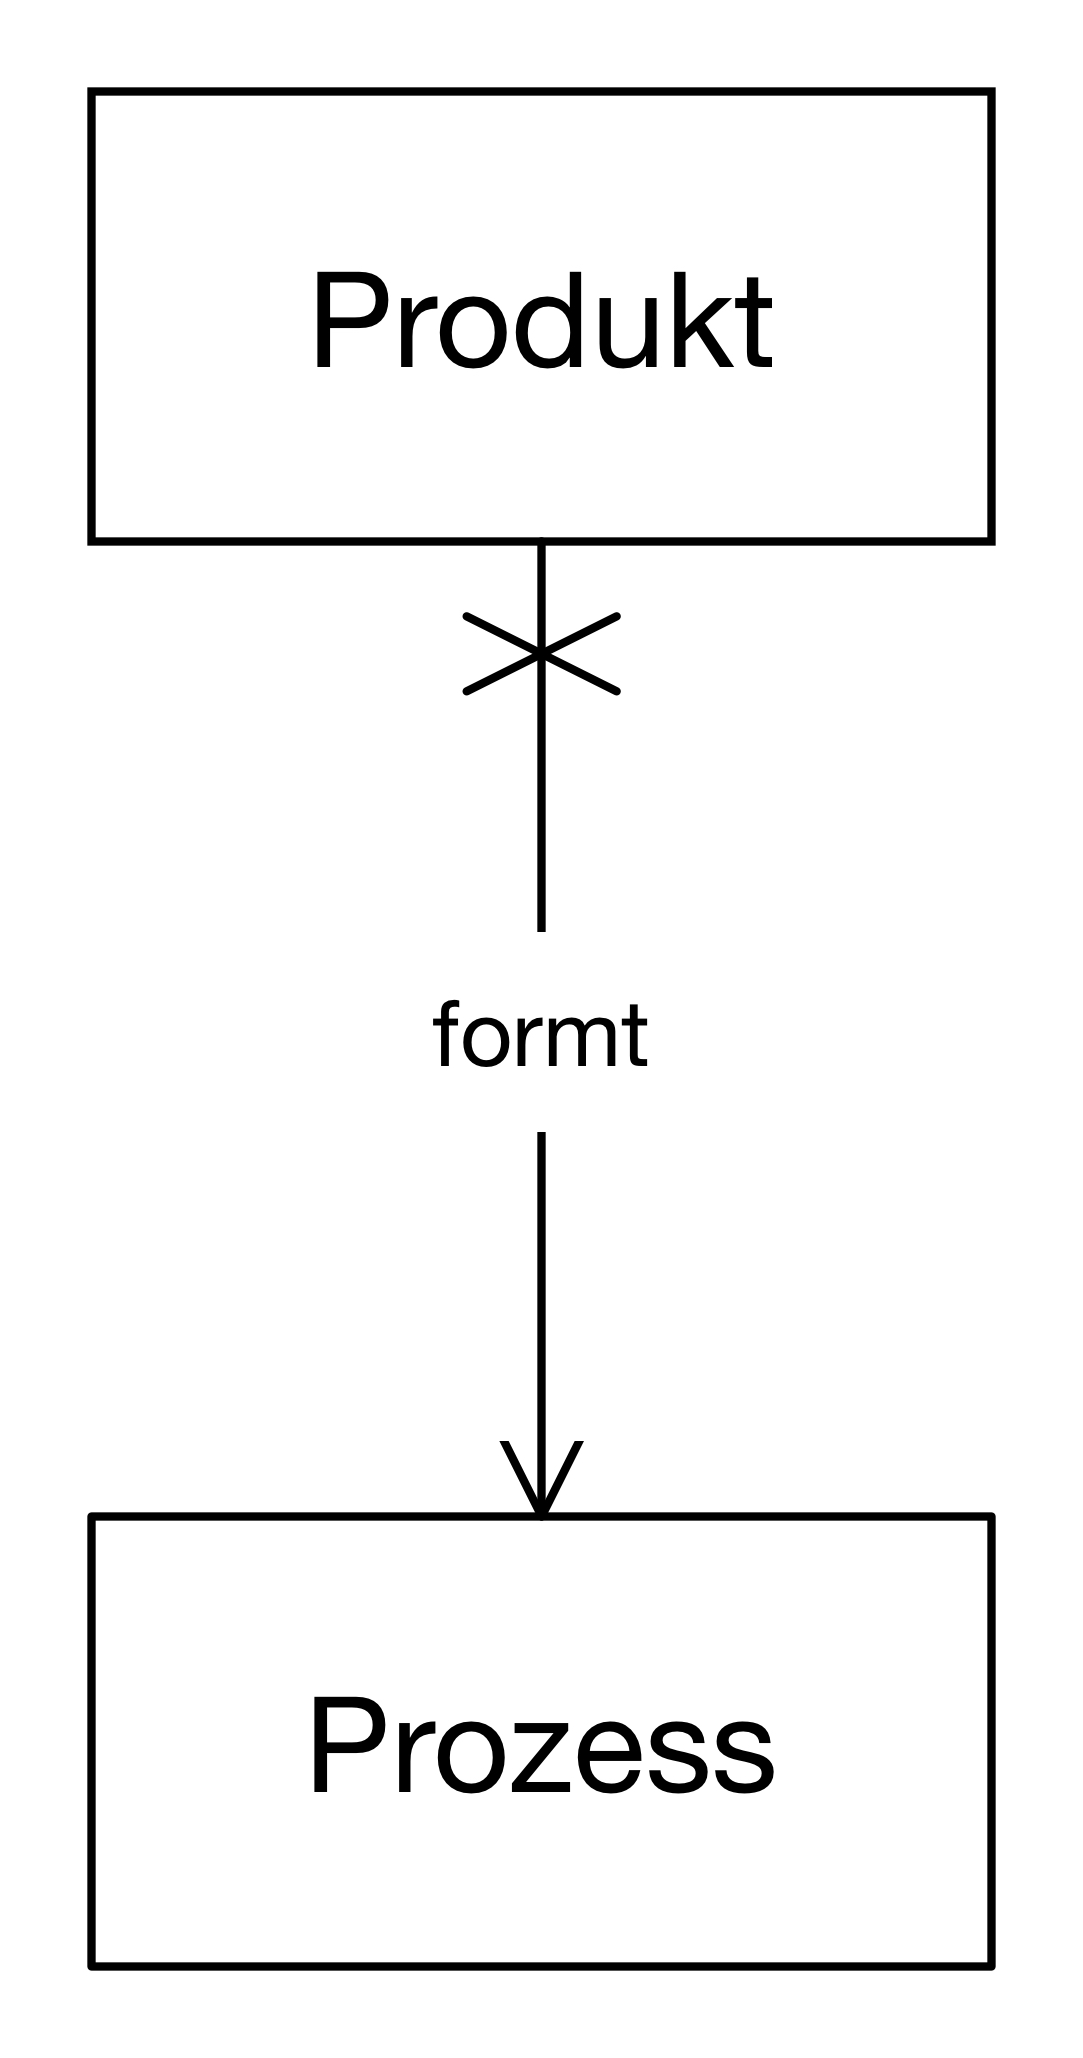
\includegraphics[height=0.5\textwidth]{graphics/stateoftheart/Prozess.jpg}
		\caption{Definition eines Prozess}
	  	\label{fig:prozessdef}		
	\end{figure}
	
	Laut der Norm \acs{DIN} \acs{IEC} 60050-351 ist ein Prozess wie folgt definiert:\\
	
	\textit{Ein Prozess repräsentiert einen Ablauf von sequentiell ausgeführten Aktivitäten innerhalb eines Systems zum Umwandeln, Lagern und Transportieren von Material, Energie oder Informationen.}\\
	
	\textit{Ein technischer Prozess ist ein Prozess, dessen physikalische Werte gemessen, sowie mit technischen Mitteln beeinflusst werden.}\cite{mpolke_proc}\\
	
	Zu unterscheiden ist zwischen folgenden Prozessen:
	
	\begin{itemize}
		\item Diskreter Prozess
		\item Kontinuierlicher Prozess
		\item Chargenprozess
	\end{itemize}
	
	\subsection{Diskreter Prozess}
	Der diskrete Prozess wird häufig auch als \glqq Fertigungsprozess\grqq\space definiert, wobei es sich dabei im Grunde genommen um dasselbe handelt. Zu den Eigenschaften solch eines Prozesses gehört ein klar definierter Start- und Endzeitpunkt. Der grundlegende Unterschied zu den noch folgenden ist jener, dass ausschließlich bei diskreten Prozessen die Formveränderung praktiziert wird, was wiederum bedeutet, dass es zu keiner stofflichen Strukturveränderung während des gesamten Ablaufs kommt. Zur Anwendung kommt diese Art in der Fertigung von mechanischen Produkten, wie etwa konkret in der Automobilindustrie.
	
	\subsection{Kontinuierliche Prozess}
	Konträr zum diskreten Prozess steht der häufig bei der Stromerzeugung zum Einsatz kommende kontinuierliche Prozess. Hierbei gibt es keinerlei festgeschriebenen Anfangs- und Endzeitpunkt, was zur Folge hat, dass an jedem Ort immer die selben Zustände auftreten, wobei der Betrachtungszeitpunkt irrelevant ist. Bei diesen oft auch als stationär bezeichneten Prozessen wird etwa zu Beginn einer Produktionskette stets der selbe Zustand des Produkts auftreten. Dabei beschränkt sich die Verarbeitung auf formlose Stoffe, die Sand, Flüssigkeiten oder Ähnliches sein können. Es kommt lediglich zu einer stofflichen Veränderung, wie einer chemischen Reaktion oder dem Aufheizen beziehungsweise Mischen mit einer anderen Substanz.
	
	\subsection{Chargenprozess}
	Bei der dritten und letzten Beschreibung handelt es sich um eine Art von Prozess, die teilweise Parallelen zu diskreten und kontinuierlichen Prozessen aufweist. So wird abermals mit formlosen Materialien gearbeitet, welche ausschließlich stofflich verändert werden. Der ausschlaggebende Unterschied zu kontinuierlichen Prozessen ist jedoch, dass es klare Anfangs- und Endzeitpunkte während des Prozesses gibt. So hat etwa das Füllen eines Tanks ein eindeutiges Endergebnis, über das nicht folgenlos hinausgegangen werden kann.\\

	Ableitbar aus den obigen Definitionen müssen Anlagen auf Basis spezifischer Prozesse geplant und erbaut werden. Die Anlage hat hingegen keinen Selbstzweck, sondern dient einzig und alleine nur dafür, einen oder mehrere Prozesse zu realisieren.\\

	% ##################################################################
	% Warum welche Hardware (Kriterien für unsere Nutzung, Umsetzbarkeit
	% ##################################################################
	\section{Hardwareaufbau einer \ac{SPS}}
	
	Um die im späteren Verlauf aufbauende Hardware genauer beschreiben zu können, muss zu Beginn ein wenig thematisch ausgeholt werden. So hat der Begriff der Steuerung einen undenkbar hohen Stellenwert, welcher ebenso geklärt gehört.\\

	Unter einer Prozess- Steuerung versteht man nach der Norm \acs{DIN} 19226 einen Vorgang, bei dem durch Rückführen gemessener Prozesszustände, verglichen mit von der speicherprogrammierbaren Steuerung formulierten Parametern, Sollwerte zur Beeinflussung des gesamten Prozesses erzeugt werden. Im Gegensatz zu einer Regelung muss der von einem Sensor ausgelesene Ist-Wert jedoch nicht zwanghaft rückgeführt werden. Dies ist in Abbildung~\ref{fig:Aufbau_Steuerkreis_Selfmade} ersichtlich.\cite{mseitz_sps}\\
	
	Der Steuerkreis besteht aus Sensoren, einem Steuerungsrechner, welcher meistens mittels einer \ac{SPS} realisiert wird, sowie Aktoren. Die Steuerungseinheit selbst ist ein Rechner mit dem Hauptaufgabenbereich, die programmierten, im Speicher abgelegten Anweisungen zyklisch auszuführen und über einfach anzusprechende Schnittstellen Daten einzulesen oder auszugeben. \cite{mseitz_sps} \\
	
	Der Begriff \ac{SPS} wird in der Norm \acs{DIN} \acs{EN} 61131-1 (\acs{IEC} 61131-1) wie folgt definiert:\\
	
	\glqq \textit{Ein digital arbeitendes elektronisches System für den Einsatz in industriellen Umgebungen mit einem programmierbaren Speicher zur internen Speicherung der anwenderorientierten Steuerungsanweisungen zur Implementierung spezifischer Funktionen wie z.B. Verknüpfungssteuerung, Ablaufsteuerung, Zeit-, Zähl- und arithmetische Funktionen, um durch digitale oder analoge Eingangs- und Ausgangssignale verschiedene Arten von Maschinen und Prozesse zu steuern. Die Speicherprogrammierbare Steuerung und die zugehörige Peripheriegerät (das \ac{SPS}- System) sind so konzipiert, dass sie sich leicht in ein industrielles Steuerungssystem integrieren und in allen ihren beabsichtigten Funktionen einsetzen lassen.}\grqq \space \cite{sps_programmierung}\\
 
 	\begin{figure}[h!]
  		\centering
      	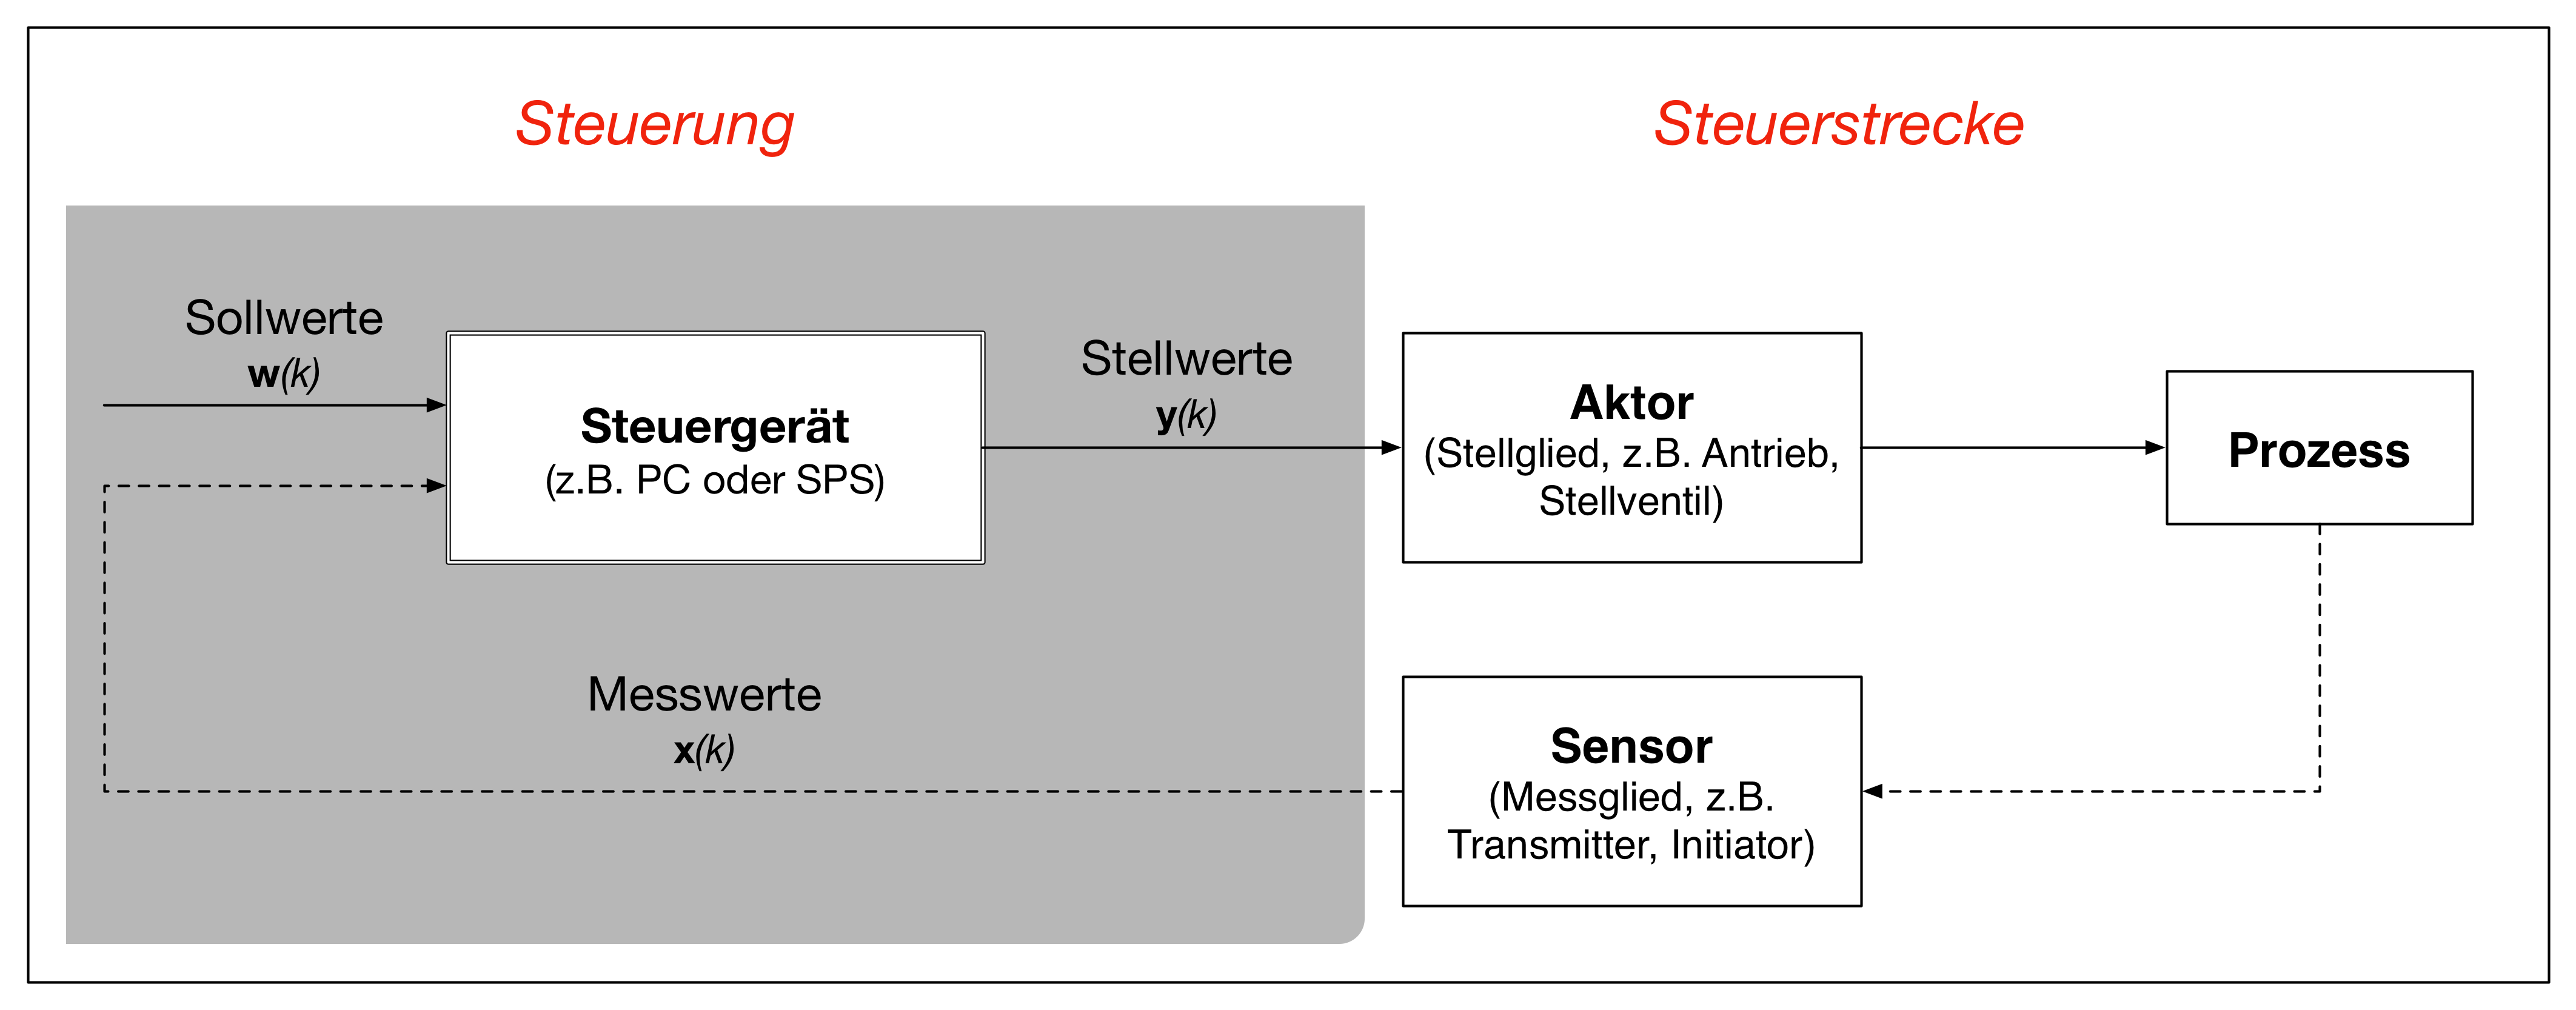
\includegraphics[width=1\textwidth]{graphics/stateoftheart/Aufbau_Steuerkreis_Selfmade.png}
  		\caption{Allgemeiner Aufbau eines Steuerkreises \cite{mseitz_sps}}
			\label{fig:Aufbau_Steuerkreis_Selfmade}
	\end{figure}	
 
 
 Im Detail gehört zum Aufbau einer \ac{SPS} eine Stromversorgung, eine Verarbeitungseinheit (\ac{CPU}), digitale sowie analoge I/O Anschlüsse, eine Feldbusschnittstelle und das Programmiergerät, wobei es sich dabei heutzutage eigentlich ausschließlich um einen externen Computer handelt. Die Stromversorgung \ac{PS} wandelt gleichzeitig die Netzspannung in eine 24-V-Gleichspannung um, mit der die Elektronik der \ac{SPS} versorgt wird.\\
	
	Man unterscheidet drei verschiedene Aufbauarten bei \ac{SPS}en
	
	\begin{itemize}
  		\item Hardware - \ac{SPS}
  		\item Slot - \ac{SPS}
  		\item Soft - \ac{SPS}
	\end{itemize}

	\textbf{Hardware - \ac{SPS}}\\\\
	Der im vorigen Abschnitt beschriebene Aufbau einer \ac{SPS} bezieht sich auf die klassische Aufbauform einer \textit{Hardware - \ac{SPS}}. Ihre Komponenten sind als gewöhnliche Einsteckkarten in einem Gehäuse oder Schaltschrank angeordnet und sind über einen Rückwandbus miteinander verbunden. Die Hardware - \ac{SPS} benötigt einen externen PC als Programmiergerät.\\
	
	\textbf{Slot - \ac{SPS}}\\\\
	Eine Slot - \ac{SPS} ist eine Einsteckkarte für den PC, welche alle Module einer \ac{SPS} enthält. Anstatt einer \ac{CPU} befindet sich ein Co-Prozessor in ihr, auf dem ein eigenes multitaskingfähiges Betriebssystem läuft. Zusätzlich verfügt sie über einen sogenannten multi-ported RAM (ein geteilter Speicher, der sowohl für \ac{SPS}, als auch für PC zugreifbar ist).\\
	
	\textbf{Soft - \ac{SPS}}\\\\
	Zu guter Letzt gibt es die Soft - \ac{SPS}, welche im Gegensatz zu den anderen Steuerungseinheiten eine reine Softwarelösung ist, die komplett auf der \ac{CPU} des Host-PCs läuft und auch deren Hardware nutzt. Zur Ankopplung der Sensoren und Aktoren ist eine Einsteckkarte zur Feldbuskopplung notwendig, die mit einem Prozessor zur Buskommunikation und einem dual-ported Ram ausgestattet ist.\\
	
	Die Vorteile der \ac{SPS} im PC ergeben sich hauptsächlich dadurch, dass die rasante Entwicklung der PC-Leistungen für \ac{SPS}en genau dafür genutzt werden kann.\\
	
	Die Informationsverarbeitung in einer \ac{SPS} verläuft zyklisch. Die Verarbeitungsschritte lassen sich vereinfacht mit dem EVA - Prinzip beschreiben.
	
	\begin{itemize}
		\item \textbf{E}inlesen der Sensordaten
		\item \textbf{V}erarbeiten der Informationen im \ac{SPS}-Programm
		\item \textbf{A}usgeben der Soll-Werte an die Aktoren
	\end{itemize}
	
	Die \ac{CPU} fragt anfangs nacheinander alle Eingangskanäle ab und legt anschließend die Daten in den Arbeitsspeicher - es entsteht das sogenannte \glqq Eingangsabbild\grqq. Hierbei handelt es sich jedoch nicht um die aktuellen, sondern um die zum Abtastzeitpunkt ausgelesenen Werte. Die erstellten Programme werden ausschließlich von der \ac{CPU} jeweils Schritt für Schritt abgearbeitet. Erst nach Abarbeitung \textbf{aller} Programme werden die im Ausgangsabbild abgelegten Sollwerte nacheinander an die Ausgangskanäle übertragen (siehe Abbildung~\ref{fig:eva}). \cite{mseitz_sps} \\ 
	
	Kleinere \ac{SPS} - Hersteller versuchen ihre eigene spezifische Hardware möglichst kompatibel für fremde Software zu produzieren, um mit ihrem Produkt eine möglichst große Zielgruppe anzusprechen. Große Hersteller hingegen möchten ihr System eher geschlossen für den Zugriff mittels fremder Software halten, um die Kundenbindung auf den verschiedensten Ebenen der Automatisierungspyramide zu erhöhen.
	
	\begin{figure}[h!]
  		\centering
    	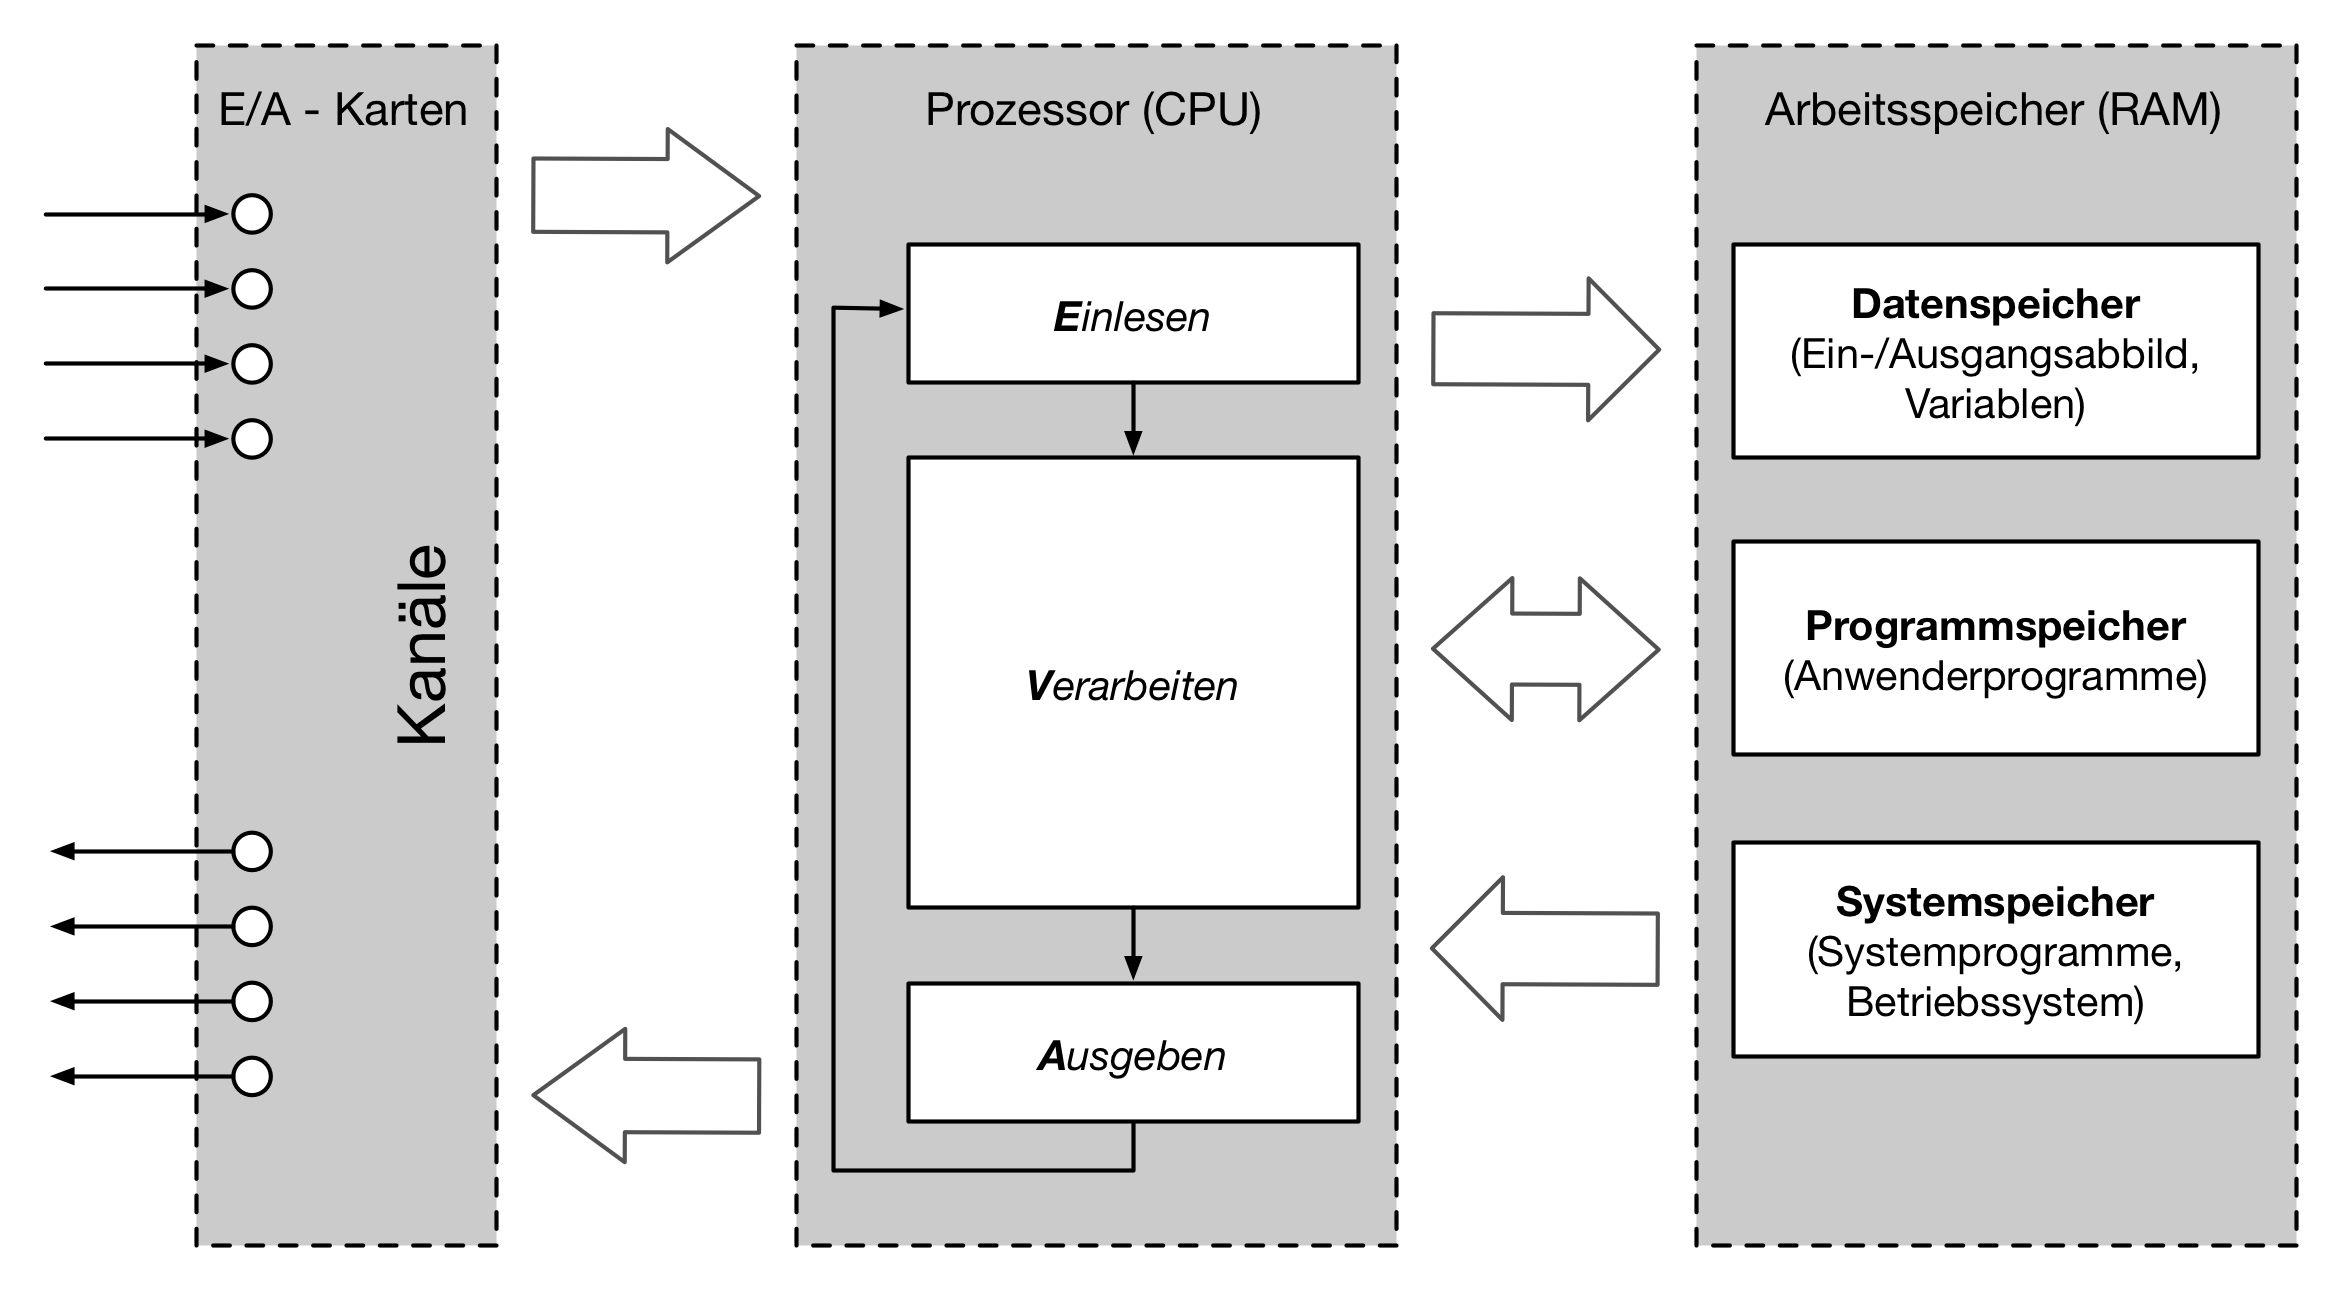
\includegraphics[width=1\textwidth]{graphics/stateoftheart/Signalverarbeitung_Selfmade.png}
  		\caption{Signalverarbeitung und Arbeitsweise einer \ac{SPS} \cite{mseitz_sps}}
  		\label{fig:eva}
	\end{figure}
		
	% ##############################################################
	% Programmierung einer SPS - Wie funktioniert das grundsätzlich?
	% ##############################################################
	\section{Programmierung einer \ac{SPS}}

	In der Automatisierungs- und Regelungstechnik gibt es zum Erfüllen der gegebenen Anforderung mehrere Wege um diese zu lösen. Genauer gesagt handelt es sich hierbei um ganze sechs verschiedene Programmiersprachen, um auf jede möglich auftretende sowie spezifische Anforderung individuell eingehen zu können. Diese unterteilen sich wiederum in zwei differenzierbare Untergruppen. So gibt es zum einen die textbasierten Programmiersprachen
	
	\begin{itemize}
		\item[1)] Anweisungsliste (engl. \textit{Instruction List})
		\item[2)] Strukturierter Text (engl. \textit{Structured Text})
		\item[3)] Ablaufsprache (engl. \textit{Sequential Function Chart})
	\end{itemize}

	Im Gegensatz dazu gibt es noch die grafikbasierten Programmiersprachen
	
	\begin{itemize}
		\item[4)] Kontaktplan (engl. \textit{Ladder Diagram})
		\item[5)] Ablaufsprache (engl. \textit{Sequential Function Chart})
		\item[6)] Funktionsbausteinsprache (engl. \textit{Function Block Diagram})
	\end{itemize}
	
	Ziel dieser Vielfalt ist es, eine Vereinheitlichung der Programmierung von \ac{SPS}en zu erreichen. Der Standard 61131 ist seit 1993 eingeführt und industriell etabliert. Mittlerweile schon in der dritten Edition verfügbar, und somit auch Objektorientierung unterstützend, sind die Programmiersprachen für zentrale und eng gekoppelte Systeme ausgelegt.
	
	\subsection{Anweisungsliste}
	Diese textbasierte Programmiersprache nach der Norm \acs{IEC} \acs{DIN} \acs{EN} 61131-3 ist sehr maschinennahe. Vergleicht man die Anweisungsliste aus Listing \ref{lst:awl} mit höheren Programmiersprachen der Informatik, so ist es eine Art Assemblersprache, die normalerweise 1:1 den jeweiligen Maschinencode übersetzt. Es werden die einzelnen Anweisungen in der Reihenfolge geschrieben, wie sie die Maschine (\ac{CPU}) abarbeiten soll (auch \glqq Stackorientierte Abarbeitung\grqq \space genannt). Ein großer Vorteil gegenüber allen grafischen Programmiersprachen ist die Tatsache, das AWL funktionell über diese hinausgeht, weil beispielsweise ein komplexer Zählvorgang mittels eines Kontaktplans nicht realisierbar sein könnte. \cite{spslehrgang_struktur, egroetsch_sps}

	\lstinputlisting[caption=Beispiel einer Anweisungsliste,label=lst:awl,style=ST]{extra/awl.txt}

	\subsection{Strukturierter Text}
	Diese anschließend angeführte Programmiersprache der Automatisierungstechnik orientiert sich an der Sprache Pascal, enthält aber neben dieser Sprache zugehörigen spezifischen Elementen aber auch noch \ac{SPS}-typische Elemente. Geeignet ist \ac{ST} am vorteilhaftesten für Aufgaben mit mathematischem Hintergrund sowie zum Beschreiben komplexer Algorithmen. Auch für Rezept- und Datenverwaltung hebt sich diese Art der Programmierung durch enorme Vereinfachung vor. Typische Anweisungen für ST sind solche, die in höheren Sprachen durch Bedingungen oder Schleifen ausgeführt werden können \cite{grundlagen_automatisierungstechnik}
	
	\lstinputlisting[caption=Beispiel eines Strukturierten Texts,style=ST]{extra/st.txt}
	
	\subsection{Ablaufsprache}
	Eine Sonderstellung unter den Sprachen zur Programmierung einer \ac{SPS} nimmt die Ablaufsprache ein. Da die Inhalte dieser entweder grafisch (siehe Abbildung ~\ref{fig:as}) oder textuell (siehe Listing~\ref{lst:as}) definiert werden, wird ein recht breit gefächertes Feld an Anwendern abgedeckt.\\

	Die eigentliche Programmierung verläuft mittels Schrittketten. Generell ist diese Art der Programmierung einer \ac{SPS} anderen Sprachen übergeordnet. Der oberste Programmablauf wird immer mittels Ablaufsprache beschrieben. Der eigentliche Programmaufbau erfolgt durch Schritte und Transitionen, die in einer gerichteten Ablaufkette zusammengefügt werden. Üblicherweise sind den Transitionen Schaltbedingungen, und den Schritten Aktionen zugeordnet. Voraussetzung für das Schalten in einen Schritt ist, dass der vorhergehende Schritt aktiv ist und die Transitionsbedingung erfüllt ist.\\

	\begin{figure}[h!]
  		\centering
    	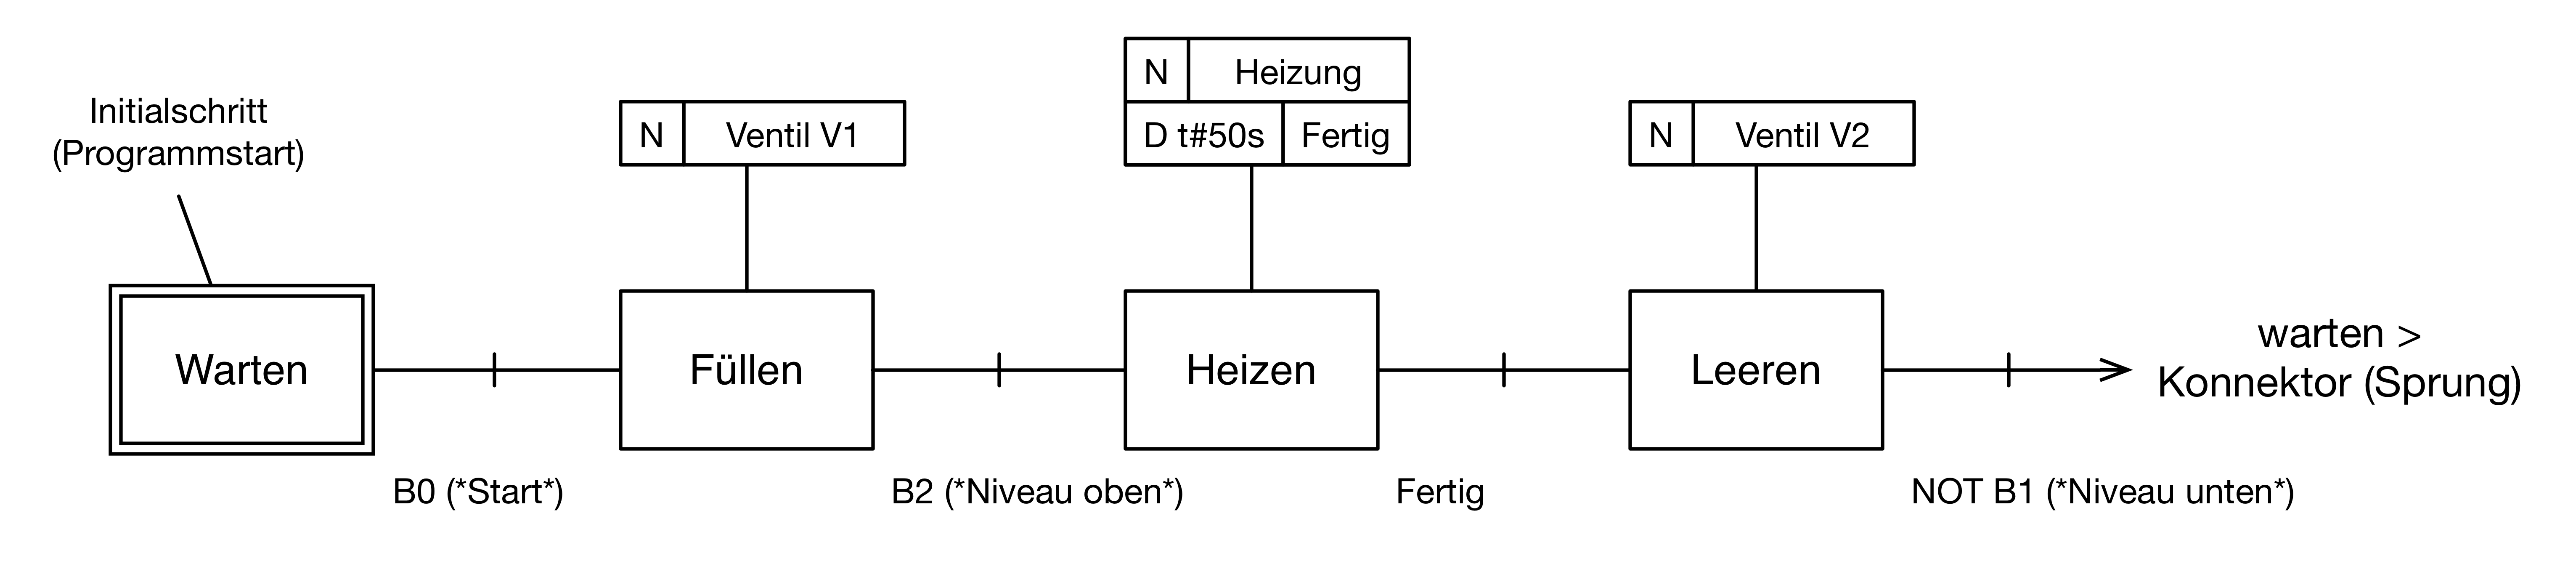
\includegraphics[width=1\textwidth]{graphics/stateoftheart/as.png}
  		\caption{Grafisches Beispiel der Ablaufsprache \cite{indsteu}}
  		\label{fig:as}
	\end{figure}
	
	\lstinputlisting[caption=Textuelles Beispiel der Ablaufsprache,label=lst:as, style=ST]{extra/as.txt}
	
	\subsection{Kontaktplan}
	Die Darstellungsart des Kontaktplans (siehe Abbildung~\ref{fig:kontaktplan}) ermöglicht \ac{SPS}-Programmierern ein Programm auf grafischer Ebene zu erstellen und darzustellen. Ein \ac{KOP} ist einem Stromlaufplan sehr ähnlich, um Programmieranfängern, die noch nie zuvor analytisch hinterfragten Code entwickelt haben, den Einstieg zu erleichtern. Es werden Elemente wie Spulen, Öffner/Schließer, Eingänge/Ausgänge, usw... verwendet, die zu logischen Blöcken zusammengefasst werden können und so einen Teil des gesamten Programms ergeben. Ein Nachteil dieser standardisierten Programmiersprache ist jedoch, dass es nicht für alle möglichen Operationen auch ein einheitliches Symbol in einem Stromlaufplan gibt. Das wiederum bedeutet, dass bei komplexen Steuerungen oft eine Mischung aus \ac{KOP} und der \ac{FBS} verwendet wird.\\

	\begin{figure}[h!]
  		\centering
    	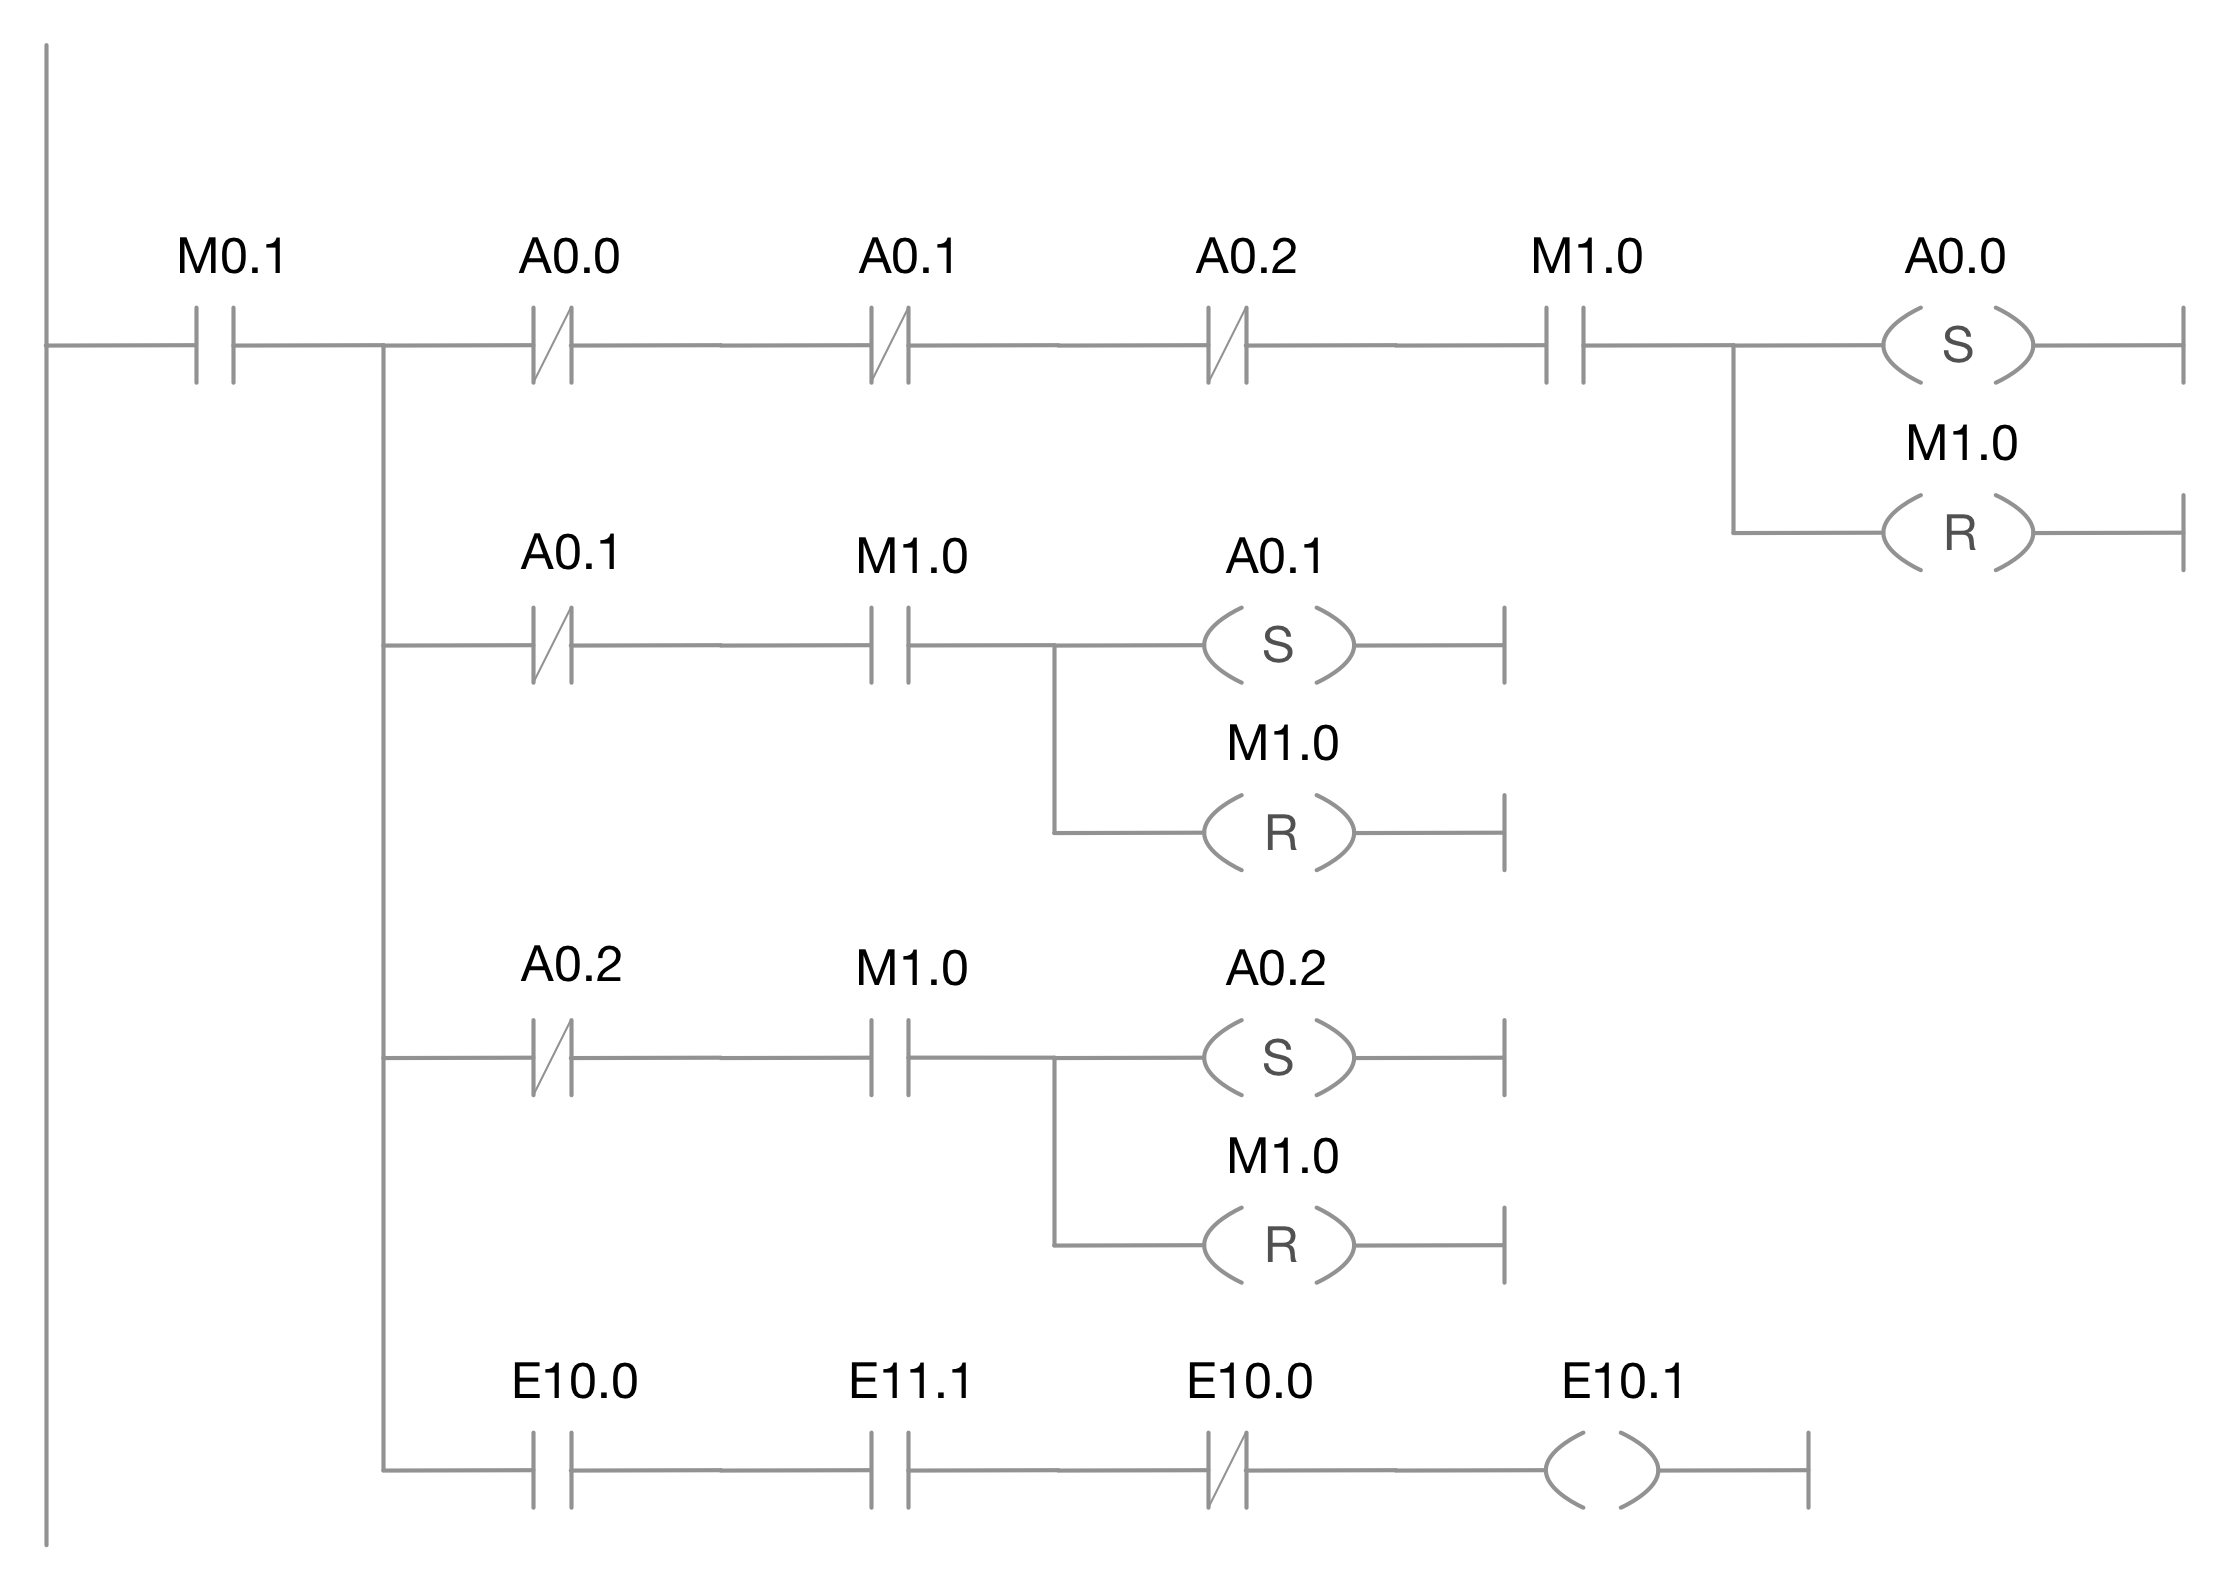
\includegraphics[width=0.8\textwidth]{graphics/stateoftheart/kop_Selfmade.png}
  		\caption{Beispiel eines Kontaktplans \cite{kontaktplan}}
  		\label{fig:kontaktplan}
	\end{figure}

	\subsection{Funktionsbausteinsprache}
	Diese grafische Programmiersprache (siehe Abbildung~\ref{fig:fup}) verwendet für ihre Anweisungen logische Symbole der Boolschen Algebra. Diese Sprache ist insbesondere für Verknüpfungssteuerungen geeignet und deswegen bei Anfängern oder Programmier - Laien beliebt. Durch den einfachen grafischen Aufbau ist die Programmlogik relativ schnell zu erkennen und nachzuvollziehen.

	\begin{figure}[h!]
  		\centering
    	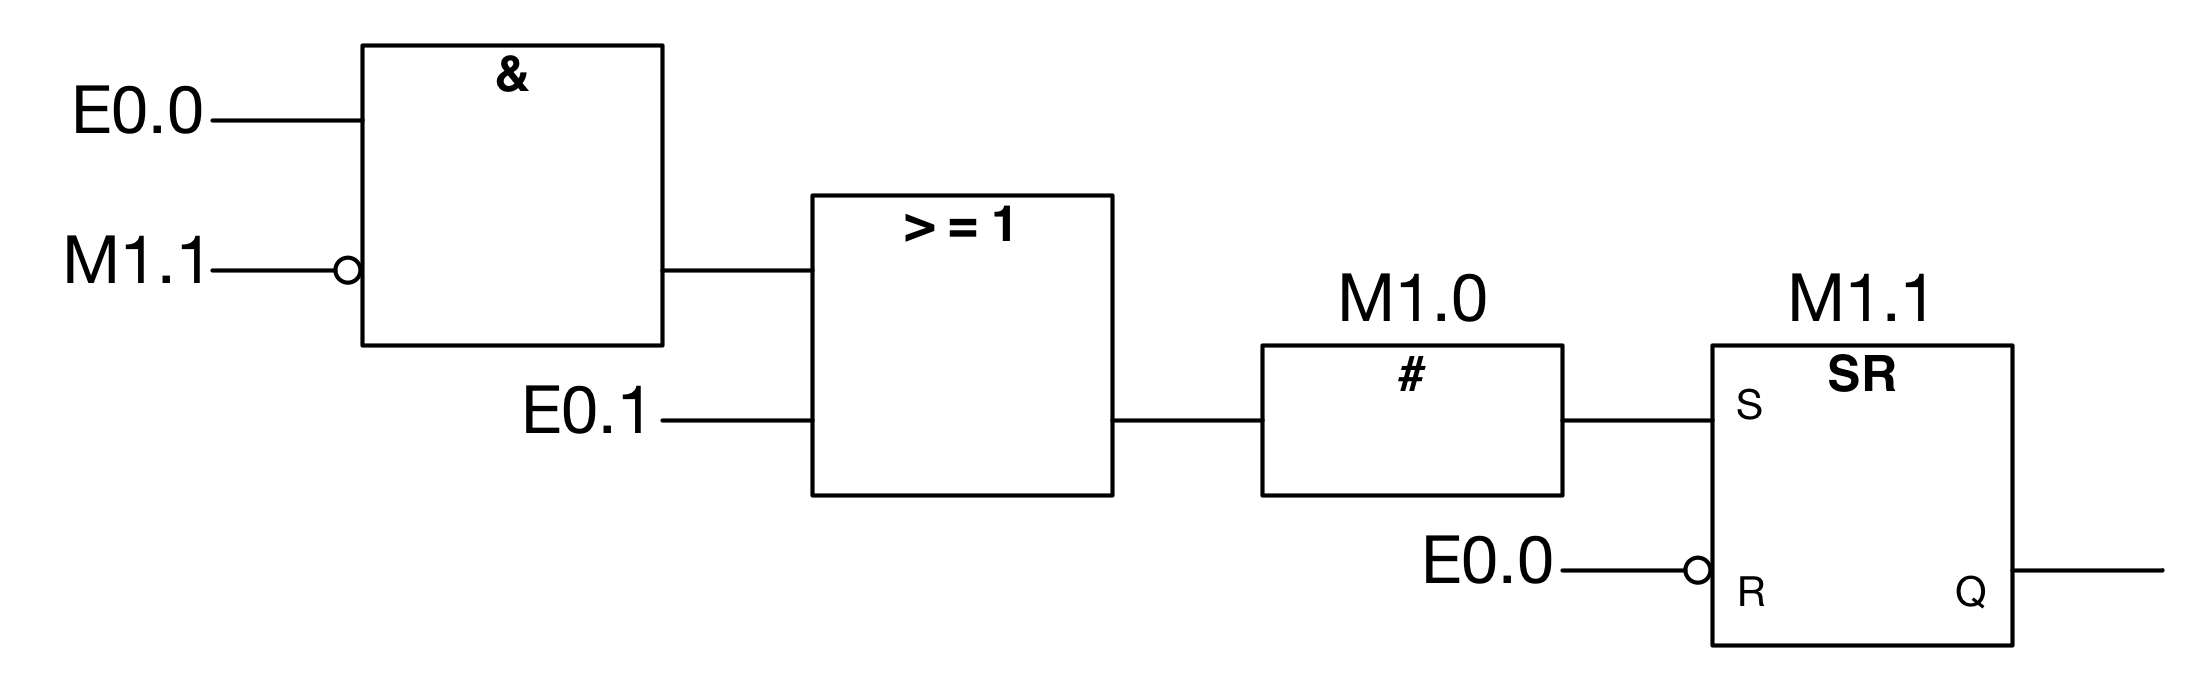
\includegraphics[width=0.8\textwidth]{graphics/stateoftheart/funktionsbausteinplan_Selfmade.png}
  		\caption{Beispiel eines Funktionsbausteinplans \cite{funktionsbausteinplan}}
  		\label{fig:fup}
	\end{figure}

\section{Prozedur}
Die Prozedursteuerung bestimmt, dass Aktionen in einer geordneten Folge stattfinden, damit eine prozessorientierte Aufgabe ausgeführt wird. Prozedursteuerungen sind charakteristisch für chargenorientierte Prozesse.\\

%Quelle EN 61522
\begin{figure}[h!]
		\centering
		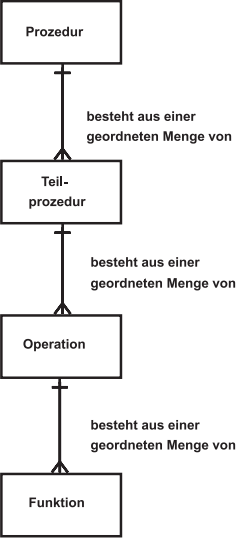
\includegraphics[width=0.3\textwidth]{graphics/stateoftheart/prozedursteuerung.png}
		\caption{Aufbau einer Prozedur \cite{en61512}}
		\label{fig:prozsteuer}
\end{figure}
\newpage

Wie in Abbildung \ref{fig:prozsteuer} ersichtlich, besteht eine Prozedur aus weiteren Teilen. Die Prozedur, sowie die Elemente die Teile einer solchen sind und deren Zusammenhänge können folgendermaßen erklärt werden:\\

\textbf{Prozedur}\\
Die Prozedur ist die höchste Stufe in der Hierarchie und legt die Strategie für die Ausführung einer umfassenden Verarbeitungsaktion, wie zum Beispiel der Herstellung einer Charge, fest. Sie wird durch eine geordnete Menge von Teilprozeduren bestimmt.\\

\textbf{Teilprozedur}\\
Eine Teilprozedur besteht aus einer geordneten Menge von Operationen, die bewirken, dass eine zusammenhängende Produktionssequenz in einer Teilanlage stattfindet. Es wird angenommen, dass zu jeder Zeit immer nur eine Operation in einer Teilanlage aktiv ist. Eine Operation wird in einer einzelnen Teilanlage vollständig ausgeführt. Gleichwohl können mehrere Teilprozeduren einer Prozedur konkurrierend ablaufen, jede in einer anderen Teilanlage.\\

\textbf{Operation}\\
Eine Operation ist eine geordnete Menge von Funktionen, die eine größere Verarbeitungssequenz festlegt und die bewirkt, dass die verarbeiteten Stoffe von einem Zustand in einen anderen überführt werden, womit gewöhnlich eine chemische oder physikalische Umwandlung verbunden ist. Häufig ist es erwünscht, die Grenzen einer Operation auf Punkte in der Prozedur zu legen, wo die normale Verarbeitung sicher ausgesetzt werden kann.\\
Beispiele für Operationen sind:
\begin{itemize}
	\item Füllen: z.B. destilliertes Wasser hinzugeben.
	\item Reaktion: Zwei Komponenten mischen, heizen und auf das Absinken des Reaktordrucks abwarten.
\end{itemize}

\textbf{Funktion}\\
Die Funktion einer Prozedursteuerung ist das kleinste Element, das eine prozessorientierte Abfolge realisieren kann. Eine Funktion kann in Subteile unterteilt werden. Der \acs{IEC} 60848 Standard definiert die Art, wie Funktionen durch Schritte und Übergenge unterteilt werden können. \\
Ein Schritt kann eine oder mehrere Anweisungen ausgeben oder eine oder mehrere Maßnahmen bewirken, zum Beispiel:
\begin{itemize}
	\item Setzen, Löschen und Ändern von Alarmgrenzen und anderen Grenzwerten.
	\item Lesen von Prozessvariablen, wie z.B. Volumendurchfluß von einem Durchflussmesser.
\end{itemize}

Das Ziel einer Funktion ist es, eine prozessorientierte Aktion zu bewirken oder zu definieren, wogegen die Logik oder die Folge von Schritten, die die Funktion ausmachen, einrichtungsspezifisch ist.\\
Beispiele für eine Funktion wären \cite{batchproc}:
\begin{itemize}
	\item Rühren
	\item Heizen
\end{itemize}

\section{Rezept}
Rezepte sind Teil der Europäischen Norm \acs{EN} 61512, welche den Aufbau bei der Chargenorientierten Fahrweise definiert.\\\\
\textit{„Ein Rezept ist eine Gesamtheit, die die Minimalmenge von Informationen enthält, die eindeutig die Herstellungsanforderungen für ein bestimmtes Produkt beschreibt. Rezepte bieten eine Methode, Produkte und die Art, wie diese Produkte hergestellt werden, zu beschreiben“.} \cite{en61512}\\\\
In der Norm werden die vier Typen von Rezepten, die fünf Kategorien von Informationen, die ein Rezept enthält und wie sich diese Information bei den verschiedenen Rezepttypen verändert, behandelt.\\\\
Es können unternehmensintern noch eigene Rezepttypen verwendet werden, falls die Definierten nicht alle benötigten Anforderungen abdecken, außerdem kann es sein, dass für ein Produkt mehrere Rezepte bestehen, wenn dieses zum Beispiel in verschiedenen Werken produziert wird und dadurch unterschiedliche Abläufe beinhaltet.\\

\subsection{Rezepttypen}
%Quelle EN 61522
\begin{figure}[h!]
		\centering
		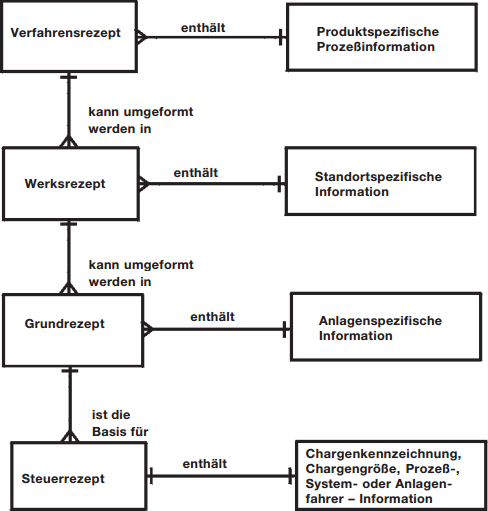
\includegraphics[width=0.6\textwidth]{graphics/stateoftheart/rezepttypen.png}
		\caption{Zusammenhang der Rezepttypen \cite{en61512}}
\end{figure}
Die verschiedenen Rezepttypen enthalten unterschiedliche viele Informationen zu Produkt und Produktionsstätte.\\\\
Die Verfahrens- und Werksrezepte beschreiben zum Beispiel nur das Prinzip, wie produziert wird während die Grund- und Steuerrezepte schon die wirklichen Betriebsmittel enthalten.
\\\\
\textbf{Verfahrensrezept}\\
Das Verfahrensrezept ist ein Rezept auf Unternehmensebene, das als Grundlage für Rezepte auf niedrigeren Ebenen dient. Das Verfahrensrezept wird ohne spezifische Kenntnis der Anlagenausrüstung erstellt, die zur Herstellung des Produktes benutzt werden wird. Es bestimmt die Rohstoffe, ihre relativen Mengen und die erforderliche Verarbeitung, allerdings ohne Bezug zu einem bestimmten Werk oder der in diesem Werk verfügbaren Ausrüstung. Es wird von Personen mit Kenntnissen der Chemie und den Verarbeitungsanforderungen erstellt, die für das betreffende Produkt typisch sind, und gibt deren Interessen und Überlegungen wieder.\\\\
Das Verfahrensrezept kann für die unternehmensweite Planung und für Investitionsentscheidungen benutzt werden. Es kann ein Teil von Produktionsvorgaben sein oder von solchen in Bezug genommen werden und kann als solches für die Produktionsplanung und zur Information von Kunden und Behörden verwendet werden.
\\\\
\textbf{Werksrezept}\\
Das Werksrezept ist spezifisch für ein bestimmtes Werk. Es ist eine Kombination von werksspezifischer Information und dem Verfahrensrezept. Es wird gewöhnlich aus einem Verfahrensrezept abgeleitet, um die Bedingungen einer bestimmten Produktionsstätte zu erfüllen, und bietet einen für werksbezogene, langfristige Produktionsplanung erforderlichen Detaillierungsgrad.
\\\\
\textbf{Grundrezept}\\
Das Grundrezept ist die Rezeptstufe, die auf eine Anlage oder eine Gruppe von Einrichtungen einer Anlage ausgerichtet ist. Ein Grundrezept kann vom Verfahrensrezept oder vom Werksrezept abgeleitet werden. Es kann mehrere von einem Werksrezept abgeleitete Grundrezepte geben, von denen jedes den Teil des Werksrezeptes abdeckt, der in einer Anlage ausgeführt werden kann. Das Grundrezept kann produktspezifische Informationen enthalten, wie sie zur detaillierten Produktionsplanung erforderlich sind, wie zum Beispiel Informationen über Prozesseinsätze oder Anforderungen an die Einrichtung.\\\\
Das Grundrezept ist eine unverzichtbare Rezeptstufe, da ohne es keine Steuerrezepte erzeugt und daher keine Chargen produziert werden können.
\\\\
\textbf{Steuerrezept}\\
Das Steuerrezept entsteht als eine Kopie einer bestimmten Version des Grundrezeptes und wird anschließend wie erforderlich durch Informationen für Dispositionsplanung und Ausführung verändert, um spezifisch für eine einzelne Charge zu sein. Es enthält produktspezifische Prozessinformationen, wie sie zur Produktion einer bestimmten Charge erforderlich sind. Es bietet den Detaillierungsgrad, wie er zum Start und zur Überwachung der Einrichtungsprozedurobjekte einer Anlage erforderlich ist. Es kann verändert worden sein, um die tatsächlichen RohstoffQualitäten und die tatsächlich eingesetzte Ausrüstung zu berücksichtigen. Die Auswahl von Teilanlagen und entsprechende Skalierung kann jederzeit durchgeführt werden, bevor diese Information benötigt wird. \cite{batchproc}\\

\subsection{Bestandteile des Rezeptes}

\textbf{Rezeptkopf}\\
Die organisatorische Information im Rezept wird als Rezeptkopf bezeichnet. Typische Informationen im Rezeptkopf kann die Rezept- und Produktidentifikation, die Versionsnummer, den Rezeptersteller, das Ausgabedatum, Freigaben, Status und andere organisatorische Angaben enthalten.
\\\\
\textbf{Stoff- und Produktionsdaten}\\
Die Stoff- und Produktionsdaten sind eine Kategorie von Rezeptinformation, die Prozesseinsätze, Prozessparameter und Prozessausstöße umfasst.
Ein Prozesseinsatz besteht aus Bezeichnung und Menge eines Rohstoffs oder eines anderen Betriebsmittels, das zur Herstellung des Produktes erforderlich ist.
Ein Prozessparameter enthält detaillierte Information wie zum Beispiel Temperatur, Druck und Zeit, die wesentlich für das jeweilige Produkt ist.  Prozessparameter können als Sollwerte, Vergleichswerte oder in logischen Bedingungen verwendet werden.
Ein Prozessausstoß besteht aus Bezeichnung und Menge eines Stoffs, die als Ergebnis einer Ausführung des Rezeptes erwartet wird.
\\\\
\textbf{Anforderungen an die Einrichtung}\\
Anforderungen an die Einrichtung schränken die Auswahl der Einrichtungen ein, die schließlich eingesetzt werden, um einen bestimmten Teil der Prozedur durchzuführen. Im Verfahrens- und im Werksrezept werden die Anforderungen an die Einrichtung typischerweise in allgemeiner Weise, wie zum Beispiel zulässigen Werkstoffen und erforderlichen Verarbeitungscharakteristika angegeben.
\\\\
\textbf{Rezeptprozedur}\\
Die Rezeptprozedur beschreibt die Strategie, um einen Prozess durchzuführen. Verfahrensrezeptprozeduren und Werksrezeptprozeduren sind unter Benutzung der im Prozessmodell beschriebenen Ebenen strukturiert, da diese Ebenen es gestatten, den Prozess in einrichtungsunabhängiger Art zu beschreiben. Grundrezeptprozeduren und Steuerrezeptprozeduren werden unter Benutzung der Prozedurelemente des Prozedurmodells beschrieben, da diese Prozedurelemente einrichtungsbezogen sind. \cite{batchproc}\\

\subsection{Einrichtungssteuerung}
Das Steuerrezept selbst enthält nicht genügend Information, um die Anlage zu betreiben. Daher wird es mit der Einrichtungssteuerung, die tatsächlich die Einrichtungen zum Betrieb und zur Produktion von Chargen veranlasst, verknüpft. Die Einrichtungssteuerung wird nicht als Teil des Rezeptes angesehen.

\begin{figure}[h!]
		\centering
		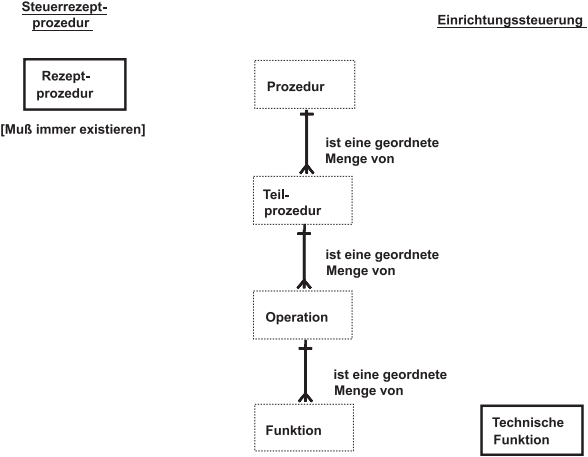
\includegraphics[width=0.8\textwidth]{graphics/stateoftheart/steuerrezeptprozedur_einrichtungssteuerung.png}
		\caption{Abgrenzung von Steuerrezeptprozedur und Einrichtungssteuerung \cite{en61512}}
\end{figure}


\section{Zenon Wizard}
Ein zenon Wizard ist ein Programm, das verwendet wird um, innerhalb der HMI SCADA Software zenon von COPA-DATA, projektspezifische Daten zu manipulieren, löschen oder erstellen. Dies kann mit oder ohne Benutzeroberfläche geschehen.\\\\
Der zenon Supervisor enthält schon bei der Installation Wizards zum Importieren sowie auch Exportieren von in \ac{XML} gespeicherten Daten und zum Erzeugen von Variablen.\cite{zenprog}\\\\
Der Quellcode der mitgelieferten Wizards kann geöffnet und auch editiert werden.\\
Zenon Wizards können mittels \ac{VSTA} oder \ac{VBA} erstellt werden. Als Beispiel zur Anwendung dieser wird in Listing~\ref{lst:vstavar} und Listing~\ref{lst:vbavar} ein Vergleich gezogen.\\\\
Außerdem kann ein selbstgeschriebener Wizard leicht mit einer benutzerfreundlichen Oberfläche verbunden werden, die in Abbildung~\ref{fig:zenwiz} dargestellt wird.

\begin{figure}[h!]
		\centering
		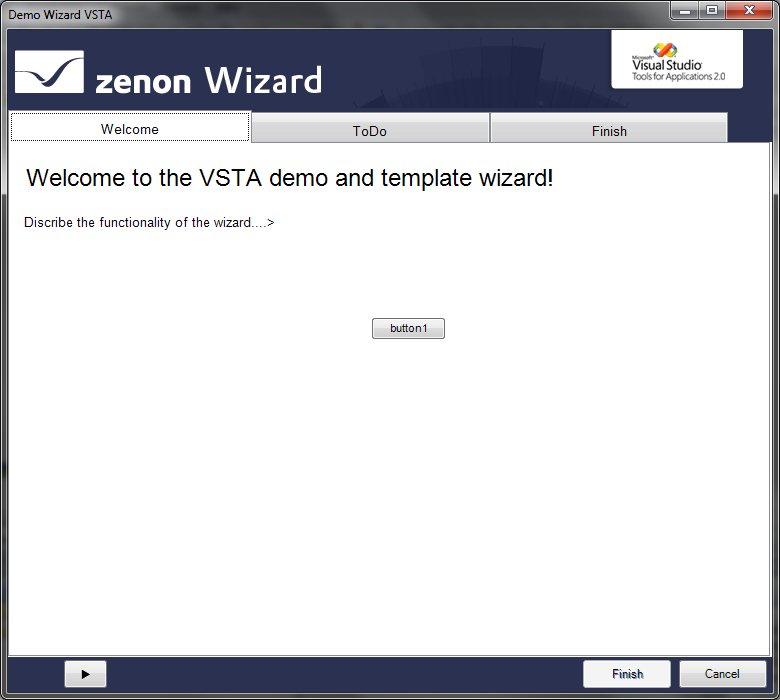
\includegraphics[width=0.8\textwidth]{graphics/stateoftheart/demowizard.png}
		\caption{Beispiel eines \ac{VSTA} Wizards}
		\label{fig:zenwiz}
\end{figure}

\subsection{\ac{VSTA}}
\ac{VSTA} ist eine Ansammlung von Werkzeugen zum erstellen von Programmen. \ac{VSTA} unterstützt die Programmiersprachen Visual Basic .Net und C\#.
\ac{VSTA} ist in Zenon als Editor integriert.

\lstinputlisting[caption=Anlegen einer Variable in C\#,style=csharp,label=lst:vstavar]{extra/sota_var_csharp.txt}

\subsection{\ac{VBA}}
\ac{VBA} steht für \textit{Visual Basic for Applications} und ist eine Skriptsprache, die dafür gedacht ist eine leichte Ontegrierung von Makros in eine Applikation zu ermöglichen. Sie wird hauptsächlich für Makros in Microsoft Office Produkten verwendet.
Ein Editor für \ac{VBA} ist in Zenon integriert.

\lstinputlisting[caption=Anlegen einer Variable in \ac{VBA},style=VBA,label=lst:vbavar]{extra/sota_var_vba.txt}

\section{Visualisierung von Produktionsanlagen}
\subsection{\ac{SCADA}}
Ein \ac{SCADA} System ist im Allgemeinen eine Sammelstelle für alle aus der Anlagen generierten Werte. Diese Daten müssen dann weiterverarbeitet werden um daraus Analysen zu erstellen.\\
Zu den Elemente eines \ac{SCADA} Systems gehören:\\
Ein \ac{SCADA} System besteht aus den folgenden 3 Teilen:\\
\\
\textbf{\ac{SCADA} Master Station Computer Systems}\\
Dies ist die Sammelstelle für Echtzeitdaten, die von RTUs generiert werden. Meist sind diese Station herkömmliche Computer.\cite{scada_system} \\ 
\\
\textbf{Remote Terminal Units (RTUs)}\\
Sensoren, die physikalische Änderungen in der Anlage mit einem Signalumformer in elektrische Werte umwandelt. Je nachdem was gemessen werden soll, entstehen analoge (Füllstand, Helligkeit, Druck, ...) oder digitale (z.B. Status eines Geräts) Werte.\cite{scada_system} \\
\\
\textbf{Human-Machine Interface}\\
Im HMI werden die gesammelten Daten der RTUs analysiert und daraus Prognosen bzw. Diagnosen Visuell aufbereitet, um den Anwender eine schnell erkennbare Anzeige zu bieten.\cite{scada_system}

\subsection{HMI}
Die Visualisierung einer Produktionsanlage ist ein wesentlicher Punkt der Datenverarbeitung und wird oft als Benachrichtigungszentrale benutzt. Meist werden in dieser mit geringer Verzögerung aktualisierte Statuswerte sowie Benachrichtigungen zu unerwarteten Ereignissen angezeigt. Die hierfür benötigten Daten müssen von der \ac{SPS} in die Visualisierungssoftware übermittelt werden. Da dies ein sehr aufwendiger Prozess ist, gibt es \ac{SCADA}-Systeme die all diese Funktionen vereinen.\\
\\
Für dieses Projekt wurde eine Umsetzung in der \ac{SCADA} Software zenon verlangt, daher wird im weiteren nur noch über die Visualisierung in zenon's HMI System, \textbf{zenon Supervisor}, gesprochen.\\
\\

\newpage

\section{Modellbasierte Entwicklung der Steuerung} \label{modellbasierte_entwicklung}
Das Gebiet der modellbasierten Entwicklung bzw. der automatisierten Codegenerierung aus einem Modell als ganzes kann nicht als State of the Art erklärt werden, da sich dieser Ansatz zurzeit noch in der Forschung befindet.\\
Allerdings können die einzelnen Gebiete dieser Entwicklung im heutigen Betrieb schon gefunden werden.
\subsection{Modell}
Ein Modell der gesamten Anlage wird schon im frühen Stadium der Entwicklung in Form eines \ac{RI} hergestellt, um klar zu definieren, welche Bauteile benötigt werden und welches mit welchem Bauteil verbunden ist. Dies ist nur das erste Modell das in der Industrie eingesetzt wird.\\
\\
Oft werden aber mehr Informationen benötigt als im \ac{RI} ersichtlich sind, weswegen man auf eine andere Methode umsteigen muss ein Modell abzubilden.\\
Auf die gängigsten Methoden (\ac{XML}, Ontologie, \ac{UML}) wird in den nächsten Punkten genauer eingegangen.
\subsection{\ac{XML}}
\ac{XML} ist eine textbasierte Modellierungssprache bzw. Dateiformat, dass obwohl es für Dokumente gedacht ist, oft für das Abbilden von Daten Strukturen verwendet wird. \ac{XML} ist wie viele andere \glqq Markup-Languages\grqq\space tag basiert, jedoch mit dem großen Unterschied das die Tags nicht vordefiniert werden, sonder die Benutzer diese erstellen. Ein wichtiger Aspekt der erwähnt werden muss ist der, das die erstellten \ac{XML} Dateien keine eigene Funktion besitzen.\\

\newpage
\lstinputlisting[style=XML,caption=\ac{XML} Beispiel Code]{extra/sample.xml}

Der Aufbau einer \ac{XML} Datei ist leicht zu erklären: Es gibt 1 rootElement, dass den Anfang und das Ende des Inhaltes markiert. Zwischen dem Start- und Endtag befinden sich weitere Tags, die das Dokument oder die Struktur genauer beschreiben. Jeder Tag kann Attribute besitzen die es weiter definieren. Zwischen einem Start- und Endtag können sich entweder weitere Tags oder einfacher Text befinden.
\\
Einsatz findet \ac{XML} meist in Programmen oder Webseiten, die größere Mengen an Daten bzw. Befehle Systemunabhängig übertragen sollen. Grund dafür ist unter anderem die Tatsache, dass Mensch und Maschine die Datei ohne Übersetzung bzw. Kompilieren lesen und verstehen kann.\\
Doch auch wenn eine Person \ac{XML}-Dateien lesen kann, dauert es länger die Struktur eines Textes, im Vergleich zu einer grafischen Darstellung, zu verstehen.\\  
Dafür gibt es andere Werkzeuge, die auf \ac{XML} basieren, aber eine grafische Darstellung erzeugen.
\subsection{Ontologie}
Eine Ontologie ist ein auf \ac{XML} basierendes Konstrukt, dass einem das Abbilden von Dingen und deren Relationen ermöglicht. Um solch komplexe Zustände darzustellen, stehen neben einfachen Entitäten (Dinge) auch Eigenschaften zur Verfügung.

\glqq ... we have at least two parts to the overall philosophical project of ontology: first, say what there is, what exists, what the stuff is reality is made out off, secondly, say what the most general features and relations of these things are. \grqq \cite{ontology_stanford} \\
\\

\textbf{Allgemeiner Aufbau einer Ontologie}\\
Das Modell an sich ohne zusätzliche Attribute oder Eigenschaften ist vom Aufbau her so zu erklären: Es gibt ein 'Thing', von dem alles aus geht, sozusagen ist das das root-Element bei \ac{XML}. Von diesem Punkt aus können weitere Entitäten abgeleitet werden, diesen Schritt kann als eine Vererbung gesehen werden. Die neu erstellte Entität ist immer noch ein Thing, jedoch genauer definiert. Es gibt keine Grenzen oder Vorschriften, in welche Tiefe diese Definition gehen muss. Daher kann dies für sehr komplexe aber auch simple Modelle eingesetzt werden.\\

\begin{figure}[hbt!]
  \centering
  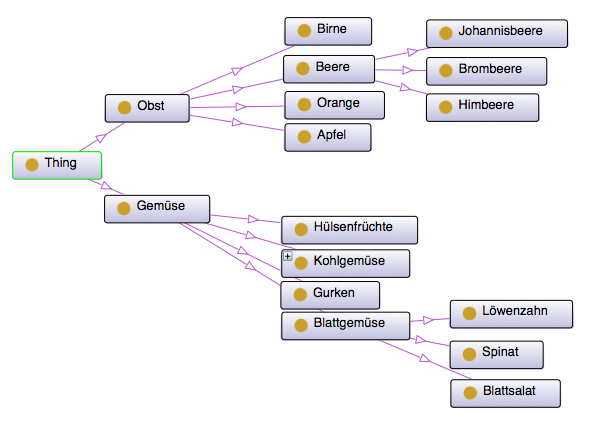
\includegraphics[width=0.8\textwidth]{graphics/stateoftheart/Ontology_example}
  \caption{Aufbau einer Ontologie}
  \label{fig:Ontology_Aufbau}
\end{figure}

Wie in Abbildung~\ref{fig:Ontology_Aufbau} erkennbar ist, erhält man so die Struktur des Modells, jedoch werden oft weitere Informationen zu den einzelnen Objekten/Entitäten benötigt, welche als Eigenschaften abgespeichert werden.\\
Dies ermöglicht ein Modell aufzubauen, dass nicht nur die Struktur abbilden, sondern komplexe Netzwerke konstruieren kann.\\
\\
\noindent \textbf{Objekt Eigenschaften}\\
Objekt Eigenschaften werden benötigt um Relationen zwischen den einzelnen Objekten genauer zu beschreiben.\\
\\
Allgemeine Definition:\\
\textbf{Domain} -> \textbf{Name} -> \textbf{Range}\\
KlasseA -> Eigenschaft -> KlasseB\\
\\
Ein Beispiel wäre eine Verknüpfung zwischen einem Tank und einer Pumpe und genau für diese Relationen gibt es Objekt Eigenschaften. Für diesen Zweck kann eine Eigenschaft mit dem Namen 'verbunden\_mit' erstellen und diese dann dem Tank beifügen. So ergibt sich die Relation:\\
\textbf{Tank -> verbunden\_mit -> Pumpe}
\\
\\
\textbf{Daten Eigenschaften}\\
Daten Eigenschaften werden benötigt um Objekte genauer zu beschreiben. 
\\
Beispiel für ein Modell einer Produktionsanlage ist es etwaige Sensoren im Modell einen Wertebereich festzulegen in welchem dieser arbeitet bzw. was für Werte dieser sammelt oder zurückgibt: Ein Füllstandsensor mit einem Wertebereich von 4-20V, wobei 4V=Leer und 20V=Voll bedeutet, kann in einer Ontologie mit wenigen Data Properties abgebildet werden.

\subsection{\ac{UML}}
\ac{UML} ist, wie eine Ontologie, eine auf \ac{XML} basierte Modellierungssprache.
Das Ziel von \ac{UML} ist es, System Architekten, Software Ingenieuren und Software Entwicklern ein Werkzeug zur Analyse, Design, Implementation von Softwarebasierenden Systemen, sowie für Modell Entwicklung und ähnliche Prozesse zu bieten.\\
\\
Mit Hilfe von \ac{UML} können viele verschiedene Arten von Diagrammen erstellt werden, für dieses Projekt relevant ist jedoch nur das Aktivitätsdiagramm, daher wird im weiteren nur auf dieses genauer eingegangen.\\
\\
%\textbf{Klassendiagramm}\\
%\\
%Neben einer einfachen Abbildung der Anlage kann man ein Activity Diagram verwenden um beispielsweise einzelne Phasen oder ganze Rezepte abzubilden.\\
%\\
\textbf{Aktivität}\\
Ein Aktivitätsdiagramm beschreibt das Verhalten von Systemen auf Grundlage von vorgegebenen Regeln. \\

\begin{figure}[hbt!]
 \centering
  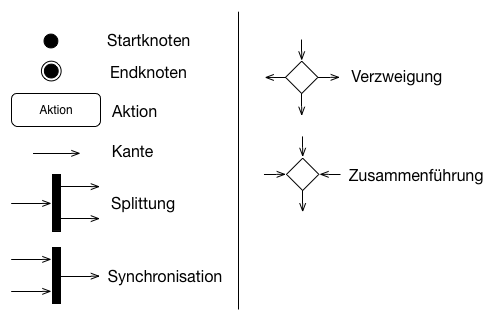
\includegraphics[width=0.8\textwidth]{graphics/stateoftheart/Activity_Elemente}
  \caption{Basis Elemente eines Aktivitätsdiagramm \cite{activity_list}}
\end{figure}

\glqq An Activity is a kind of Behavior that is specified as a graph of nodes interconnected by edges. A subset of the nodes are executable nodes that embody lower-level steps in the overall Activity. Object nodes hold data that is input to and output from executable nodes, and moves across object flow edges. Control nodes specify sequencing of executable nodes via control flow edges. Activities are essentially what are commonly called “control and data flow” models. Such models of computation are inherently concurrent, as any sequencing of activity node execution is modeled explicitly by activity edges, and no ordering is mandated for any computation not explicitly sequenced.\\
Activities may describe procedural computation, forming hierarchies of Activities invoking other Activities, or, in an object- oriented model, they may be invoked indirectly as methods bound to Operations that are directly invoked. Activities may be applied to organizational modeling for business process engineering and workflow. In this context, events often originate from inside the system, such as the finishing of a task, but also from outside the system, such as a customer call. Activities can also be used for information system modeling to specify system level processes.\\
\\
\textbf{Activity Nodes}\\
ActivityNodes are used to model the individual steps in the behavior specified by an Activity.\\
\\
\textbf{Activity Edges}\\
An ActivityEdge is a directed connection between two ActivityNodes along which tokens may flow, from the source ActivityNode to the target ActivityNod.\grqq \cite{UML_def} \\

\begin{figure}[hbt!]
 \centering
  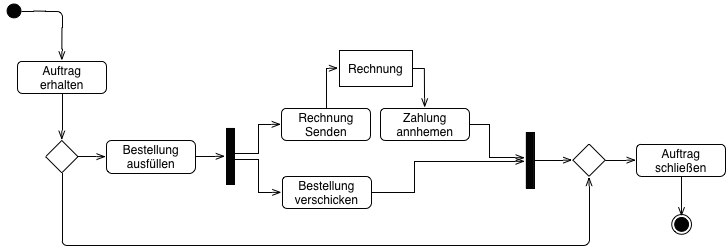
\includegraphics[width=0.9\textwidth]{graphics/stateoftheart/Activity_bsp}
  \caption{Beispiel für ein Aktivitätsdiagramm \cite{activity_example}}
\end{figure}
 
\clearpage
\section{Zusammenfassung}

Dieses Kapitel zeigt die Entwicklung und den aktuellen Stand der Technik bezüglich der Anlagen- und Verfahrenstechnik sowie der modellbasierten Entwicklung von Steuerungen für Produktionsanlagen. \\\\
Wie sich herausgestellt hat, ist die Codegenerierung für \ac{SPS}en in Produktionsanlagen heutzutage nicht State Of the Art. Bei Änderungen wie dem Hinzufügen oder Entfernen von Teilen muss ein Großteil des Programm-Codes neu implementiert werden. \\\\
%Um eine Codegenerierung für \ac{SPS}n in Produktionsanlagen  
%„“
Die Idee ist, diesen Implementierungsschritt auf einer Laboranlage zu automatisieren. Der \ac{SPS} Code soll einerseits auf einem Ontologie-basierten Informationsmodell, um das Produktionssystem abzubilden, und andererseits auf einem Aktivitätsdiagramm, um die Prozeduren zu definieren, generiert werden.
Wenn es nun zu Änderungen der Produktionsanlage kommt, können diese im Modell angepasst werden und durch eine Codegenerierung der nötige Implementierungsschritt automatisiert werden. Zusätzlich wird die Integrierbarkeit des Codes in eine Steuerungsapplikation mit Visualisierung mittels der Software zenon von COPA-DATA getestet werden.\\\\
Im Rahmen des Projekts Batch\_it soll eine Laboranlage konzeptioniert und aufgebaut werden. Darüber hinaus wird eine Steuerungsapplikation mit Visualisierung mithilfe der Software zenon erstellt werden. Dies umfasst das Implementieren von Prozeduren und Rezepten nach dem \acs{IEC} 61512 Standard. Hierbei handelt es sich um Funktionen wie z.B. das Pumpen von Flüssigkeiten von Tank zu Reaktor. Im letzten Schritt wird die modellbasierte Entwicklung der Steuerung umgesetzt. Dabei wird einen Ontologie erstellt, welche die Laboranlage abbildet und ein Aktivitätsdiagramm, welches die Prozeduren definiert. Anhand dieser wird einen Codegenerierung für die Steuerung der Anlage mittels des zenon Wizards implementiert.\\\\
\textbf{Forschungsfragen}\\\\
%Mit welchen Technologien ist die Implementierung von Code einer \ac{SPS} einer Chargenprozessanlage automatisierbar? \\\\
Wie genau muss die Chargenprozessanlage abgebildet werden um eine Codegenerierung zu ermöglichen? \\\\
Welche Funktionalitäten der Steuerung kann durch die modellbasierte Entwicklung der Steuerung abgedeckt werden?\\\\
Wie ausführlich funktioniert die Integrierung der Codegenerierung in die Software zenon von COPA- DATA? 